%AUTOR: František Horázný

\chapter{Úvod}

Tato práce využívá zpracování zvukových signálů pro výpočet přibližné polohy řečníka v~prostoru. Zpracování signálů je využíváno v~mnoha odvětvích: úprava zvuku pro komerční účely, příjem a vysílání signálu z~mobilních telefonů, příjem signálu ze satelitu pro televize jsou jen některé příklady. Tato práce se zabývá zpracováním zvukového signálu od řečníka. Zpracování zvukového signálu je rozšířený obor využívaný v~múzických uměních, v~telekomunikacích, v~systémech reagujících na slovní povely, při tovární výrobě aerodynamických předmětů a podobně. Využití signálů k~určení polohy zdroje používá například armáda ve formě sonarů a radarů.

Cílem práce je analyzovat oblasti nutné pro porozumění problému určení pozice řečníka v~prostoru. Využitím získaných informací navrhnout a implementovat algoritmus pro výpočet pozice řečníka. Posléze upravit algoritmus tak, aby mohl běžet v~čase na dodaném hardwaru. A~porovnat přesnosti programu bez omezení a po optimalizaci.

Lokalizace zdroje takového zvuku se může využívat v~řečnických místnostech pro automatický záběr kamer nebo reflektorů. Může se však využít i při špionáži a určit při odposlechu, kde stojí odposlouchávaná osoba.

V~kapitole \ref{Teorie} je shrnuta veškerá nutná teorie využita při zpracování zvuku. V~další kapitole \ref{metody} je úvod do problematiky využití signálů pro určení polohy. Dále v~kapitole \ref{Návrh} jsou popsány komponenty využité pro vypracování aplikace, návrh řešení a úpravy nutné pro běh v~čase. Další kapitola \ref{testovani} ukazuje výsledky testování jednotlivých částí. V~kapitole \ref{experimenty} je ukázaná funkčnost aplikace jako celku na reálných datech a vlivy ovlivňující výsledné určení polohy. Na závěr jsou shrnuty výsledky, jsou uvedena doporučení pro nejlepší funkčnost aplikace a jsou navrhnuty další kroky pro další vývoj.

\chapter{Teorie} 
\label{Teorie}

V~této kapitole je popsaná nutná teorie využitá při výpočtu pozice zdroje zvuku z~nahrávaného signálu. Obsahuje vzorce, které jsou využívány v~dalších kapitolách.

\section{Zvuk}

Zvuk je mechanické vlnění, přenášené v~látkovém prostředí a projevuje se jako oscilující změna tlaku. Ve vakuu se zvuk nešíří. Vzniká vibrací pružné látky, která svým pohybem mění tlak kolem sebe, tento tlak se dále šíří tak zvaným podélným vlněním. \cite{zvuk}

Má tyto vlastnosti:
\begin{itemize}
\item Frekvenci – kolikrát za sekundu se tento tlak změní (Hz), odpovídá výšce tónu.
\item Intenzita – jak velký tento tlak je (dB), odpovídá hlasitosti.
\end{itemize}

Nejjednodušší zvukový signál má tvar funkce sinus, která je určená frekvencí (tónem) a amplitudou (intenzitou). Takto generovaný signál můžeme označit jako harmonický. Harmonický signál je jakýkoli signál opakující stejný vzorek v~čase. Zvuk se neskládá pouze z~tónu jedné frekvence. Obvykle se skládá z~více respektive mnoha dalších tónů a šumu. Šum však nedokážeme rozložit na jednotlivé složky. Vzniká například jako elektrický šum, kdy samovolně v~elektronice mírně kolísá napětí a tím mění výsledný signál zachycený z~mikrofonů. Je to náhodný signál bez jakékoli vazby na sledovaný zvuk.

Rychlost šíření zvuku není v~každé látce stejná, závisí na hustotě a teplotě látky. Například ve vzduchu se šíří mnohem pomaleji než v~kovu. Nás zajímá pouze rychlost šíření ve vzduchu. Tato rychlost se dá vypočítat vztahem:

\begin{equation}
	v=\sqrt{\frac{\gamma R T}{M}},
	\label{sireni_zvuku}
\end{equation}

kde $\gamma$ je poissonova konstanta, $R$ je molární plynová konstanta (J/mol K), $T$ je teplota plynu (K) a $M$ je molární hmotnost plynu (mg/mol). \cite{rychlost}

Dosazením za konstanty $\gamma = 1,4$, $R=8,314$ \cite{konstanty} a proměnnou $M=28,95$, získáme rovnici:

\begin{align}
	v~&= \sqrt{\frac{1,4\cdot 8,314\cdot T}{0,02895}}, \\
	v~&= 20,05 \sqrt{T}.
	\label{sireni_zvuku}
\end{align}

Tento vzorec zanedbává změny molární hmotnosti, která je závislá převážně na tlaku, ale také na složení vzduchu. Některé zdroje (\cite{rychlost}) také uvádí vzorec zjednodušující nárůst rychlosti zvuku na lineární funkci. Tento vzorec je dostatečně přesný v~rozmezí přibližně od -30 \degree C do 30 \degree C. Vychází z~přesného výpočtu rychlosti při teplot 20 \degree C (331,37 m/s) a při 1 \degree C (331,97 m/s) a zapíše se následovně:

\begin{equation}
	v=331,37 + 0.6 T,
\end{equation}

kde T je teplota ve \degree C. Tento vzorec se může v~různých zdrojích mírně lišit podle proměnných použitých v~rovnici, jako je například molární hmotnost, která je závislá i na tlaku a složení vzduchu. Pro tuto práci je důležitá rychlost zvuku v~běžném tlaku (1 bar) a teplotě kolem 20 \degree C.  V~těchto podmínkách vychází rychlost zvuku po zaokrouhlení stejně v~obou těchto vzorcích a to 343 m/s.%která je po zaokrouhlení 343 m/s při použití obou z výše uvedených vzorců.

\section{Hlas a sluch}
\label{hlas a sluch}

Jedním z~prostředků k~dorozumívání živočichů je vydávání zvuků. Schopnost lidí komunikovat pomocí hlasu, řeči, zpívání, křiku nebo šeptání je v~živočišné říši jedinečná. Vzduch vytlačovaný z~plic rozechvívá hlasivky uložené v~hrtanu a vzniká zvuk, který jazyk a rty modelují ve slova. Na modelování zvuku, který vychází přes hlasivky, se také podílí hltan, zuby, nosní a lebeční dutiny. Hlasivky jsou blány napnuté v~hrtanu. Na tyto blány jsou napojené svaly, které je napínají nebo povolují. Silně napnuté blány vytvářejí vysoké tóny, mírně povolené vytváří hluboké tóny. Celý tento proces je řízen centrem v~mozkové kůře v~levé části mozku. Maximální frekvence hlasu může být až 10 kHz, ale to pouze u~vytrénovaného jedince. Obvyklé frekvence potřebné k~dorozumění jsou do 3 kHz.  
Pro zpracování řeči je potřeba tyto zvuky zachytit. K~tomu slouží jeden ze smyslů, sluch. Jeho základem je zachycení, zpracování a vedení zvukových signálů.  Zvukovou vlnu zachycuje ušní boltec a směřuje jí do zvukovodu až k~bubínku. Bubínek je blanka, která se zvukem rozechvěje a funguje jako rezonátor. Zvukovou vlnu předává dál přes tři sluchové kůstky do vnitřního ucha. Ve vnitřním uchu se mimo jiné nachází stočená trubice (hlemýžď) naplněná tekutinou – endolymfou.  Chvění endolymfy rozvibruje vláskové buňky, které předávají vzruch sluchovým nervem do mozku ke zpracování.  Při podráždění vláskových buněk dochází k~uvolňování kationtů a nervovému impulsu. Sluchový orgán transformuje mechanické vlnění plynným prostředím přes tekuté prostředí na elektrickou energii pomocí chemických procesů. \cite{encyklopedie} \cite{hlasasluch}

Mozek nezpracuje pouze přenášené informace, ale také přibližnou polohu zdroje zvuku. K~této lokalizaci je nutné mít minimálně dva přijímače, tedy ušní boltce. Jestliže detektory zvuku jsou všesměrné, pak nelze určit polohu zdroje zvuku. Tomu napomáhá natočení ušních boltců a zkušenost. Člověk dokáže například poznat, zda se jedná o~zvuk letadla nebo zvířete a podle zkušeností a intenzity zvuku odhadne vzdálenost zdroje. Díky dvěma senzorům dokáže člověk určit úhel a odhadnout polohu zdroje zvuku. Problém však nastává například při odrážení zvuku, jako tomu je například u~zmiňovaném letu letadla. Zvuk přichází majoritně z~jiného místa, než na kterém se letadlo opravdu nachází. To je způsobeno odrazy od jakékoli překážky v~cestě zvuku. Tento odraz je označován jako ozvěna případně dozvuk.

Rozsah slyšení u~člověka je 16 až 20 000 Hz. Existuje oblast, kdy ucho je nejcitlivější. U~člověka je to 1000–3000 Hz. V~této frekvenci jsou zvuky dětského pláče nebo volání o~pomoc, pro člověka zvuky nejdůležitější. Sluch je jedním z~nejdůležitějších smyslů, varuje před nebezpečím, umožňuje komunikaci. Lidský sluch v~porovnání se sluchem jiných živočichů je na nízké úrovni. Nejcitlivější sluch ze suchozemských živočichů mají netopýři. Létají za tmy a orientují se pomocí echolokace. Vysílají zvuk o~vysoké frekvenci, odražené zvukové vlny zachycují a opakováním těchto signálů zaměřují předmět v~prostoru.  Jsou schopni vnímat a vysílat signály o~frekvenci až 212000 Hz. Dokonale vybaveny pro zaměřování zdroje zvuku jsou sovy. Jejich sluch jim umožňuje v~absolutní tmě přesně lokalizovat kořist. Uši u~sov nejsou vidět, nemají ušní boltce. Vztyčená pírka u~některých sov napomáhají k~zachycení zvukových vln. U~ušního otvoru mají dvě kožní řasy, přední řasu mohou vztyčovat a slouží k~zachycení zvuků zezadu. Ušní otvory jsou velké lasturovité. Díky asymetričnosti sluchového aparátu dokáží sovy určit i přesnou polohu kořisti. Sovy využívají k~lokalizaci časové rozdíly mezi pravým a levým uchem, který je pouze 4milisekundy. Sova je schopna od sebe odlišit dva zdroje zvuku vzdálené 1,6\degree ve vodorovném směru, stejně tak je schopna i ve svislém směru rozlišit zdroje zvuku s~přesností 1\degree. Sova registruje i ty nejtišší zvuky, protože má extrémně velký bubínek, který zesiluje zvuk až 40krát, pro porovnání u~člověka jen 18krát. \cite{sovy} \cite{zver}

\section{Záznam zvuku a interpretace}

Záznam zvuku probíhá za pomocí mikrofonů, které mění zvukové vlny na elektrické impulsy. Většina mikrofonů funguje podobně jako ucho, tedy obsahují membránu. Tato membrána svým pohybem vytváří změny elektrického napětí, které odpovídají amplitudám signálu. Výjimkou jsou piezoelektrické mikrofony, které obsahují piezoelektrické krystaly vytvářející malý elektrický náboj na základě své deformace \cite{mikrofony}.

Tento analogický signál je poté nutné transformovat A/D převodníkem do digitální podoby. Převod z~analogového (spojitého) signálu na digitální (diskrétní) probíhá vzorkováním. Vzorkovat lze jakoukoli frekvencí, v~digitálním signálovým zpracování se však nejčastěji používají frekvence 8 kHz, 16 kHz, 24 kHz, 32 kHz, 44,1 kHz a 48 kHz.

Mikrofony, stejně jako například zvuková karta, mají svůj frekvenční rozsah, který umožňují zaznamenat. Proto je nutné uvést, jaké citlivosti je třeba dosáhnout.

Pokud budeme vycházet z~předchozí podkapitoly \ref{hlas a sluch} zjistíme, že potřebujeme zaznamenat minimálně rozsah do frekvence 3 kHz. Tyto frekvence můžeme zaznamenat pouze pokud budeme vzorkovat podle Nyquistův-Shannonova vzorkovacího teorému \cite{teorem} alespoň dvakrát vyšší frekvencí, než je nejvyšší frekvence obsažená v~zachyceném signálu. Tedy zvuk o~maximální frekvenci 3 kHz musíme vzorkovat alespoň 6 kHz.

\section{Mikrofonní pole}

Mikrofonní pole je soubor dvou nebo více mikrofonů. Například se využívá ke zpracování zvuku v~lepší kvalitě. Nahrávky se nejdříve navzájem posunou a následně se sečtou. Sečtení dvou signálů je součet každých dvou sobě odpovídajících hodnot a vznikne nový signál. Tímto součtem se amplitudy zvuku sečtou a náhodný šum se navzájem vyruší nebo alespoň ztiší. Tomuto zpracování se říká tvarování (beamforming), který je popsán v~sekci \ref{beamforming}. Mikrofonní pole se může také využít k~zaměření se na určitou polohu v~nahrávaném prostoru, kde obdobně se sečtou nahrávky s~předem známým posunem, tím se zesílí zvuk z~určitého místa a ostatní zdroje se ztiší. Nejdůležitější pro tuto práci je opačné použití, tedy zjištění posunu nahrávek a tím možná detekce pozice zdroje zvuku.

Mikrofonní pole může být sestaveno z~různých počtů mikrofonů a může mít různé schéma. Základním druhem je lineární mikrofonní pole, kde jsou mikrofony řazeny na přímce. Je to jediné možné pole ze dvou mikrofonů. Další možností je rovinné pole, na které potřebujeme alespoň tři mikrofony, které spolu tvoří rovinu. Poslední možností je prostorové, kdy jsou čtyři mikrofony poskládány tak, aby každá kombinace tří mikrofonů tvořila jinou rovinu (například poskládány do tetraedru / čtyřstěnu / trojbokého jehlanu). Na obrázku \ref{pic:mikrofonni_pole} jsou tato rozestavění znázorněna.

\begin{figure}[hbt]
	\centering
	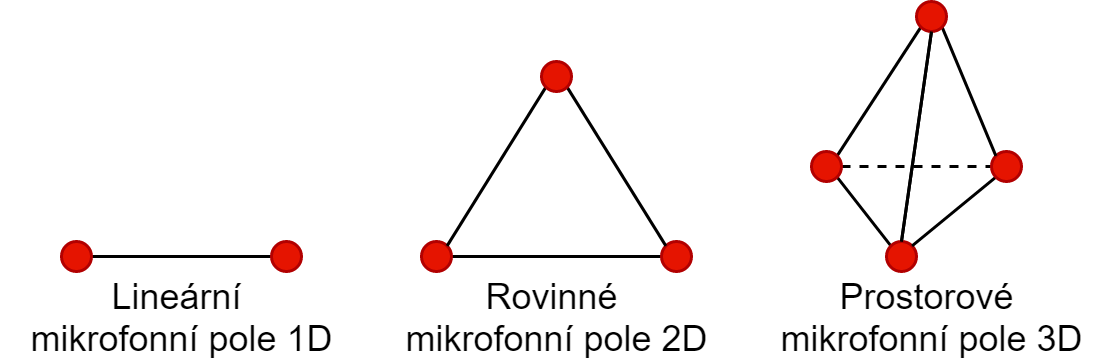
\includegraphics[width=0.6\textwidth]{obrazky-figures/mikrofonnipole.png}
	\caption{Příklady primitivních mikrofonních polí.}
	\label{pic:mikrofonni_pole}
\end{figure}

Dále je možné dělit mikrofonní pole na uniformní a neuniformní. Uniformní mikrofonní pole jsou sestavena z~mikrofonů stejně vzdálených od sebou. Neuniformní mikrofoní pole mají vzdálenosti mezi sebou různé (toho lze využít například na potlačení aliasingu, který je popsán v~dalším odstavci).

U~mikrofonních polí vzniká, stejně jako při vzorkování spojitého signálu, aliasing zachyceného signálu. To znamená, že pokud neplatí vztah \ref{eq:alias}, nelze s~jistotou určit posun těchto signálů.

\begin{equation}
	d<\frac{\gamma}{2},
	\label{eq:alias}
\end{equation}

kde $d$ je vzdálenost dvou mikrofonů a $\gamma$ je vlnová délka neovlivněná aliasingem \cite{aliasing}.

To platí pouze u~harmonických signálů, které by byly delší než porovnávané okno. Tento problém je více popsán a rozebrán i s~příklady v~sekci \ref{aliasing}.

\section{Filtrace zvuku}
\label{filt}

Digitálním filtrem se rozumí jakýkoli algoritmus, který ze vstupního signálu vytvoří upravený výstupní signál. 

Při pořízení zvuku bychom v~ideálním případě chtěli, aby nahrávka obsahovala pouze hlas. Čeho lze dosáhnout například filtrováním nahrávky. Pokud víme, že zvuk obsahuje šum o~neidentifikované frekvenci a hlas o~frekvenčním rozsahu od 16 Hz do 10 kHz, chceme všechny ostatní frekvence ideálně odfiltrovat. 

Toho lze dosáhnout pásmovou propustí (band-pass filter). Pásmová propusť se dá realizovat jako spojení dolní propusti (low-pass filter) a horní propusti (high-pass filter). Filtr horní propusti lze implementovat jako výpočet i-té hodnoty signálu takto:

\begin{equation}
	y_i=\alpha y_{i-1} + \alpha (x_i-x_{i-1}),
	\label{highpass}
\end{equation}

kde $y$ je výstupní signál, $x$ je vstupní signál a $\alpha$ je vyhlazovací faktor (smoothing factor), který se pro horní propusť vypočítá:

\begin{equation}
	\alpha=\frac{1}{2 \pi \Delta_T f_c + 1},
	\label{alphahigh}
\end{equation}

kde $f_c$ je mezní frekvence (cut-off frequency) a $\Delta_T$ je čas mezi vzorky neboli:

\begin{equation}
	\label{deltat}
	\Delta_T=\frac{1}{f_s},
\end{equation}

kde $f_s$ je vzorkovací frekvence.

Filtr dolní propusti lze zapsat následovně:

\begin{equation}
	y_i=\alpha x_i + (1 - \alpha) y_{i-1},
	\label{lowpass}
\end{equation}

kde $y$ je výstupní signál, $x$ je vstupní signál a $\alpha$ je vyhlazovací faktor. $\alpha$ se vypočte pro dolní propusť:

\begin{equation}
	\alpha=\frac{2 \pi \Delta_T f_c}{2 \pi \Delta_T f_c + 1}
	\label{alphalow}
\end{equation}

kde $f_c$ je mezní frekvence (cut-off frequency) a $\Delta_T$ je čas mezi vzorky.

\section{Energie a síla signálu}

Energie signálu je důležitá vlastnost audiosignálu, protože udává jeho intenzitu. Pokud je signál hlasitější, má vyšší amplitudu a tím i větší energii. Frekvence zvuku ji nijak neovlivňuje. Ticho má energii minimální (obsahuje pouze energii šumu). Energie se vypočítá jako skalární součin sebe samého. Vzorec pro výpočet energie:

\begin{equation}
	E=\sum_{n=0}^{N-1}|x[n]|^2,
	\label{energie}
\end{equation}

kde $E$ je energie, $N$ je délka signálu a $x$ je posloupnost hodnot diskrétního signálu \cite{energie}. Energie se využívá pro detekci řeči v~signálu. Pokud signál rozdělíme na více částí (oken), lze podle prahu energie poznat, kdy toto okno obsahuje řeč a kdy obsahuje pouze šum.
\\

Síla signálu (power) se vypočítá z~energie:

\begin{equation}
	P=\frac{E}{N},
	\label{power}
\end{equation}

kde $P$ je síla, $E$ je energie a $N$ je počet vzorků diskrétního signálu \cite{energie}.


\section{Korelace signálů}

Korelace je míra podobnosti dvou signálů. Čím podobnější signály, tím vyšší korelační koeficient. Toho lze využít při zjišťování podobnosti dvou signálů, nebo při zjišťování posunutí dvou signálů vůči sobě navzájem. Posunutí lze zjistit tak, že vypočítáme korelaci pro všechny možné posuny a vybereme maximální hodnotu. Výpočet korelačního koeficientu dvou signálů lze zapsat takto:

\begin{equation}
	(f \star g)[n]=\sum_{m}f[m+n]g[m],
	\label{korelace}
\end{equation}

kde $f$ a $g$ jsou porovnávané signály a n je posun signálů \cite{korelace}.

Můžeme si všimnout, že pokud bychom počítali korelaci neposunutého signálu $f$ sama se sebou, dostaneme energii signálu. Pokud bychom počítali korelaci signálu $f$ se signálem $\frac{f}{2}$, dostaneme výslednou korelaci poloviční i když se signály jeví téměř totožné pouze s~rozdílnou hlasitostí. Proto existuje takzvaná normovaná korelace \cite{normcorel}:

\begin{equation}
norm\_corr(x,y)=\frac{\sum_{n=0}^{N-1} x[n]\cdot y[n]}{\sqrt{\sum_{n=0}^{N-1} x[n]^2 \cdot \sum_{n=0}^{N-1} y[n]^2}}
	\label{norm_korelace},
\end{equation}

kde $x$ a $y$ jsou porovnávané signály.

Za pozornost stojí podobnosti prvků v~děliteli s~\ref{energie}. Této podobnosti je využito v~implementaci a vzorec se dá tedy přepsat následovně:

\begin{equation}
norm\_corr(x,y)=\frac{x \star y}{\sqrt{E(x) * E(y)}},
	\label{norm_korelace_energie}
\end{equation}

kde $E(x)$ je energie signálu $x$ a $E(y)$ je energie signálu $y$.

Tento vzorec vypočte korelaci normovanou. Výsledná hodnota bude nabývat hodnot v~intervalu -1 až 1, kde 1 značí totožný signál. Hlasitost signálů s~tímto algoritmem bude moci být jakákoli. Normovaná korelace signálu $f$ a $f/2$ bude $1$.

Další možnost je nejdříve znormalizovat oba signály a pak spočítat běžnou korelaci využitím vzorce \ref{korelace}. Normalizace jde dosáhnout například vydělením každého prvku průměrnou hodnotou signálu.

Jinou možností korelace je GCC-PHAT \cite{gcc}, neboli generalizovaná křížová korelace s~fázovou transformací (Generalized Cross Correlation with Phase Transform):

\begin{equation}
G_{PHAT}(f)=\frac{X_i(f)[X_j(f)]^*}{|X_i(f)[X_j(f)]^*|}
	\label{gcc_korelace}
\end{equation}

kde $X_i$ a $X_j$ jsou Fourierovi transformace dvou vstupních signálů a operace $[\ ]^*$ je komplexní konjugace. Výsledný posun získáme jako maximum z~inverzní Fourierovi transformace výpočtu \ref{gcc_korelace}.

Korelaci lze provést i například pomocí odečítání hodnot signálu. Jestliže každé dva signály mezi sebou odečteme, pak jejich rozdíly udávají, jak jsou signály rozdílné. Zde je však nutnost signály nejdříve normalizovat. Vzorec pro tuto metodu:

\begin{equation}
sub\_corr(x,y)=\sum_{n=0}^{N-1} |x[n]-y[n]|.
	\label{sub_korelace}
\end{equation}

\section{Hyperbola}

Pomocí hyperbol je možné vypočítat relativně přesné souřadnice polohy zdroje zvuku. V~této sekci je popsána hyperbola obecně a její využití je rozebráno dále v~sekci \ref{Hyperbolická metoda}.

Hyperbola je kuželosečka. Pro každý bod hyperboly platí, že absolutní hodnota rozdílu vzdáleností od dvou pevně daných bodů je vždy stejná \cite{hyperbola} tedy: 

\begin{equation}
||F_1 B|-|F_2 B||=||F_1 A|-|F_2 A||.
	\label{hyp_def}
\end{equation}

\begin{figure}[hbt]
	\centering
	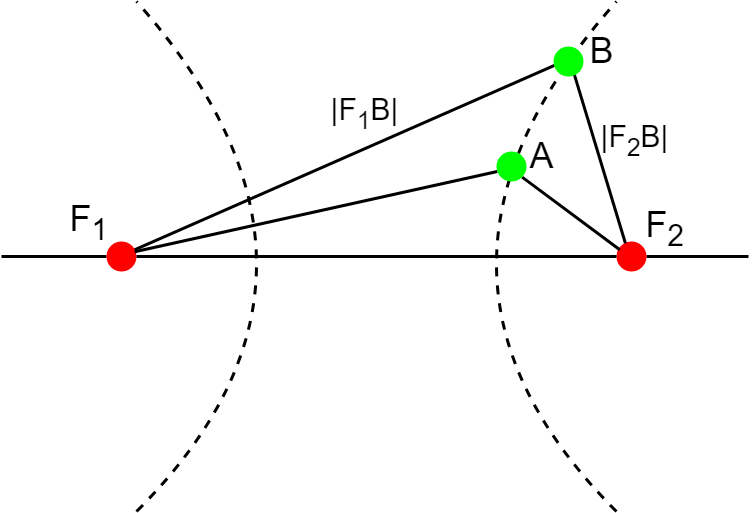
\includegraphics[width=0.6\textwidth]{obrazky-figures/hyperbola_def.png}
	\caption{Znázorněná hyperbola a na ní 2 různé body se stejným rozdílem vzdáleností od ohnisek.}
	\label{pic:hypdef1}
\end{figure}

Rovnice hyperboly lze zapsat následovně \cite{hyperbola}:

\begin{equation}
	\frac{(x-m)^2}{a^2}-\frac{(y-n)^2}{b^2}=1,
	\label{rovnice_hyperbola}
\end{equation}

kde $m$ a $n$ jsou souřadnice středu hyperboly, $a$ je hlavní poloosa hyperboly a $b$ je vedlejší poloosa hyperboly, jak je vidět na obrázku \ref{pic:hypdef2}.

\begin{figure}[hbt]
	\centering
	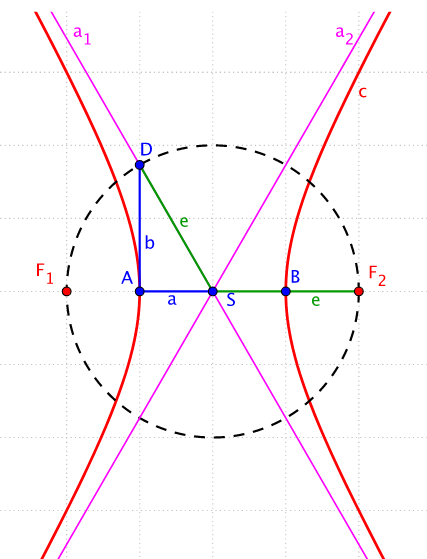
\includegraphics[width=0.5\textwidth]{obrazky-figures/hyperbola_def2.png}
	\caption{Hyperbola s~popisem excentricity, hlavní poloosy, vedlejší poloosy a středu S. převzato z~\cite{hyperbola}}
	\label{pic:hypdef2}
\end{figure}

Pythágorovou větou je možné vypočítat $b$ jako: 

\begin{equation}
    b = \sqrt{e^2 - a^2}
    \label{eq:vedlejsipoloosa}
\end{equation}

 a výpočet průniku dvou hyperbol z~dvou rovnic o~dvou neznámých:

\begin{align}
    \label{eq:prusecik}
    \frac{(x-m_{1})^2}{a_{1}^2}-\frac{(y-n_{1})^2}{b_{1}^2}&=1, \\
    \frac{(x-m_{2})^2}{a_{2}^2}-\frac{(y-n_{2})^2}{b_{2}^2}&=1.
\end{align}

Upravení této rovnice a využití je popsáno dále v~sekci \ref{navrh implementace}.

\chapter{Metody využitelné pro určení pozice zdroje zvuku}
\label{metody}

Metod pracujících se senzory přijímajícími zpožděné signály je více. Existují metody aktivní, jako například je sonar nebo radar. Tyto metody využívají odrazu vyslaného signálu od překážky a doby mezi a doby mezi vysláním a přijmutím signálu. Tímto způsobem lze zjistit vzdálenost objektu a směr. A~metody pasivní, které pracují na základě analýzy na základě přijatého signálu a rozdílu jejich dopadu. Příklad metody s~více zdroji signálu je TOA (čas příchodu – time of arrival), využívá synchronizace času na vysílačích a posílání časového razítka na jeden přijímač, který následně z~těchto údajů může zjistit svou polohu, například systém GPS. V~tomto případě se snažíme určit pozici přijímače. Cíl této práce je naopak určit pozici vysílače za využití více přijímačů neboli konkrétně mikrofonního pole.

\section{Metoda tvarování přijímací charakteristiky}
\label{beamforming}

Metody, často označované jako tvarovače (beamformer) používají upravování a sčítání jednotlivých kanálů k~zesílení konkrétní složky v~nich. Například při znalosti pozice zdroje zvuku můžeme vypočítat zpoždění jednotlivých kanálů a pak je filtrovat a sečíst. Nejjednodušší metodou je DAS (Delay and Sum – zpozdi a sečti), která pouze signály posune a sečte. Pomocí této metody lze nalézt posun takový, který má nejvyšší energetickou hodnotu. Tento signál lze považovat za posun s~nejvyšším korelačním koeficientem. Znázornění postupu výpočtu dvou různých signálů je vidět na obrázku \ref{pic:DAS}. U~této metody nelze lokalizovat více různých zdrojů, protože je brán vždy jeden nejsilnější. Při určité úpravě však můžeme zaznamenat u~každého posunu jeho energii a poté označit lokální maxima a tím získat všechny zdroje zvuku. Tato úprava může bohužel velmi lehce podléhat prostorovému aliasingu.

\begin{figure}[hbt]
	\centering
	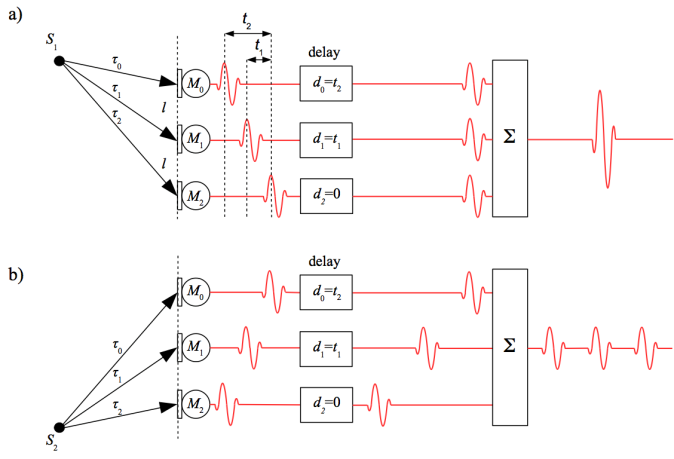
\includegraphics[width=0.7\textwidth]{obrazky-figures/DAS.png}
	\caption{Znázornění a) příchodu signálu z~místa s~očekávaným zpožděním a sečtení signálu do vyšší amplitudy. b) příchod zvuku z~místa s~neočekávaným zpožděním a rozprostření signálu. Obrázek přejat z~\cite{dasobrazek}}
	\label{pic:DAS}
\end{figure}
\newpage
\section{Metoda časového zpoždění TDOA}

TDOA (Time Difference Of Arival – časový rozdíl příchodu) je metoda lokalizace zdroje zvuku vycházející z~faktu, že v~mikrofonním poli jsou mikrofony na různých místech, a tudíž signál přichází na jednotlivé senzory s~různými zpožděními. Tato metoda využívá možnosti korelace signálů a následný výpočet ze získaných zpoždění. Zpoždění však může být buďto používáno ve výpočtu hyperbol nebo výpočtu úhlů. Ve své práci jsem se zaměřil na výpočet hyperbol, protože díky této metodě lze určit polohu zdroje zvuku v~souřadném systému. Tato metoda není schopná určit pozici více zdrojů zvuku naráz. Lze toho dosáhnout jen stejnou úpravou jako u~\ref{beamforming} metody DAS, kdy výši korelace zaznamenáme a posléze vybereme všechna lokální maxima. Znovu je důležité si uvědomit, že tuto úpravu může znehodnotit prostorový aliasing.

\subsection{Využití TDOA pro výpočet úhlů}

Při zjednodušujícím předpokladu, že zdroj zvuku se nachází v~dostatečné vzdálenosti abychom mohli předpokládat šíření zvuku po rovnoběžkách, můžeme vypočítat úhel dopadu. Tímto způsobem nelze vypočítat polohu zdroje, ale pouze směr. Pro výpočet pozice v~souřadném systému by bylo nutné zjistit vzdálenost zdroje od senzorů. Vzorec pro výpočet úhlu:

\begin{align}
    \label{eq:uhel}
    \Delta d =& \frac{N}{F_s}c, \\
    \varphi =& arcsin(\frac{\Delta d}{d_{12}}),
\end{align}

kde $\Delta d$ je rozdíl dopadu signálů na mikrofony, $N$ je zpoždění signálu, $F_s$ je vzorkovací frekvence, $c$ je rychlost zvuku, $\varphi$ je úhel dopadu a $d_1_2$ je vzdálenost mezi mikrofony.

\begin{figure}[!htpb]
	\centering
	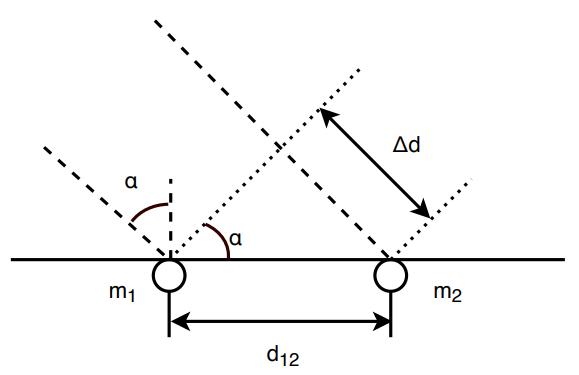
\includegraphics[width=0.5\textwidth]{obrazky-figures/TDOAuhel.png}
	\caption{Ilustrace k~rovnici \ref{eq:uhel}. Převzato z~\cite{chu}.}
	\label{pic:uhel}
\end{figure}

Tento výpočet je znázorněn na obrázku \ref{pic:uhel}, který byl převzat včetně informací v~této sekci z~\cite{chu}. Tato metoda je v~citovaném zdroji dobře popsaná, a navíc i implementovaná a testovaná. Neurčuje pozici řečníka v~souřadném systému, a proto nebyla předmětem mé práce.

\subsection{Využití TDOA a hyperbol pro výpočet souřadnic polohy}
\label{Hyperbolická metoda}

Tato metoda výpočtu pozice zdroje zvuku využívá zpoždění signálu mezi mikrofony. Vychází ze samotné definice hyperboly, tedy že pokud jsou 2 pevné body (mikrofony v~ohniscích hyperboly), pak hyperbola opisuje všechny body se stejným zpožděním. To znamená, že pomocí dvou mikrofonů lze zjistit hyperbolu, na které leží zdroj zvuku. Je však nutné si uvědomit, že hyperbolou si pouze zjednodušujeme výpočet, ve skutečnosti leží zdroj na rovině vytvořené rotací této hyperboly. Dvěma mikrofony tedy zjistíme rovinu, na které leží zdroj zvuku. Pokud použijeme tři mikrofony na jedné přímce, můžeme určit kruh kolem této osy. Obrázek \ref{pic:TDOA1} ukazuje vypočítané body lineárním mikrofonním polem se třemi mikrofony při zjednodušení na rovinný výpočet. Obrázek \ref{pic:TDOA2} ukazuje kruh, kde se zdroj zvuku může nacházet v~prostoru.

\begin{figure}[hbt]
	\centering
	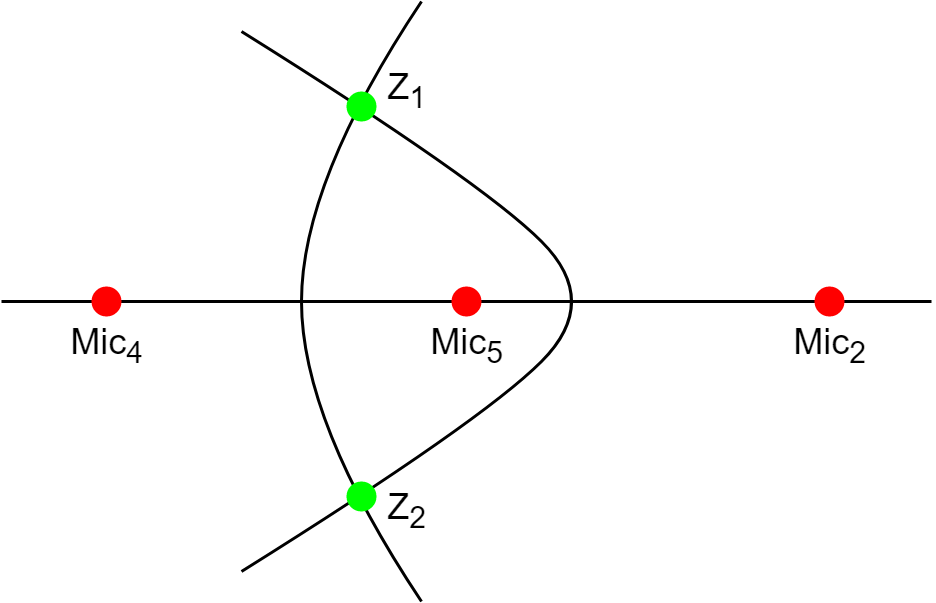
\includegraphics[width=0.7\textwidth]{obrazky-figures/TDOA_hyperboly.png}
	\caption{Vypočtené zdroje zvuku Z1 a Z2 z~lineárního mikrofonního pole ve 2D.}
	\label{pic:TDOA1}
\end{figure}

\begin{figure}[hbt]
	\centering
	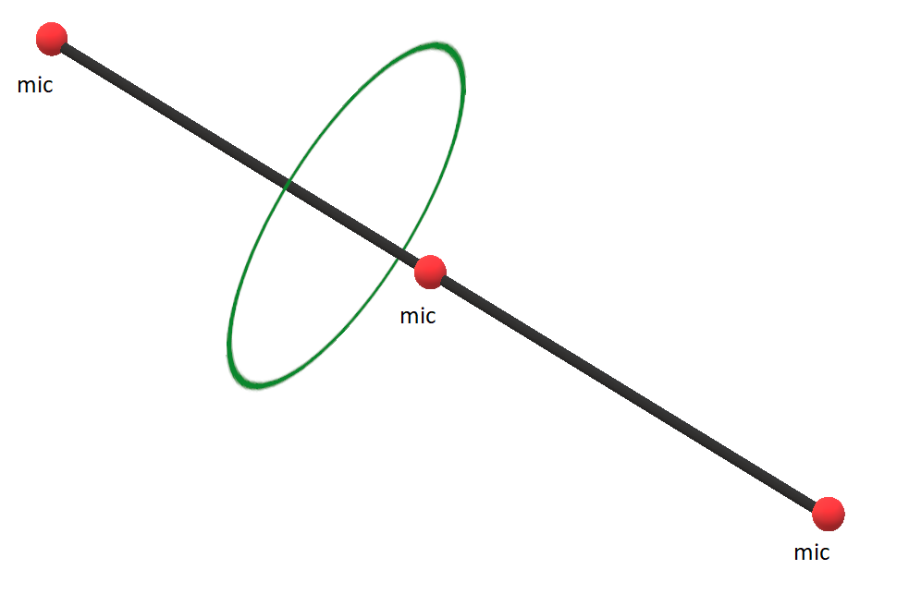
\includegraphics[width=0.7\textwidth]{obrazky-figures/TDOA_kruh.png}
	\caption{Vypočítaná možná poloha zdroje zvuku pomocí lineárního mikrofonního pole znázorněná ve 3D.}
	\label{pic:TDOA2}
\end{figure}

\newpage

Pro výpočet souřadnic polohy je vhodné použít prostorové mikrofonní pole. Pro zjednodušení lze využít rovinné mikrofonní pole, u~kterého metoda vypočítá dva body, jeden před a jeden za rovinnou mikrofonního pole. Tento problém eliminujeme například připevněním mikrofonního pole na stěnu a předpokladem možnosti výskytu zdroje zvuku pouze na jedné straně mikrofonního pole.

\chapter{Návrh řešení detekce pozice zdroje zvuku} 
\label{Návrh}

Z~předchozích kapitol vyplývá jaké algoritmy je možné použít. V~této části je řešena implementace a upravení některých vzorců, které jsou potřeba k~dosažení výsledku. Pro běh programu je nutné mít data, která se získávají pomocí půjčeného hardwaru. V~kapitole je popsán tento hardware, schéma implementovaného programu pro výpočet na laptopu, a nakonec nutné úpravy pro chod programu na zvukové kartě a slabším procesoru.

\section{Hardware}

Popis zapojení a specifikace jednotlivých komponent zapojených v~celém systému: mikrofony a mikrofonní pole, zvuková karta a laptop.

\subsection{Mikrofony a mikrofonní pole}

Pro zpracování zvuku je nutné ho zaznamenat mikrofony. Mikrofonů bylo k~dispozici 9, ale vzhledem k~nižší kvalitě nahrávky, nebyly některé z~nich použity. Byly využity elektretové mikrofony s~kulovou směrovou charakteristikou. Fotografie mikrofonu je na obrázku \ref{pic:detail_uchyceni}. Více o~typech mikrofonů viz \cite{mikrofony}. Ideální by bylo použít mikrofony s~kardioidní směrovou charakteristikou, vzhledem k~tomu, že tyto mikrofony jsou směrovější a citlivější. Sestavené mikrofonní pole předpokládáme, že bude přilehlé ke zdi. Proto vzhledem ke své směrové charakteristice by byly tyto mikrofony vhodnější. K~nahrávání bylo použito pět mikrofonů s~kulovou směrovou charakteristikou, sestaveny do kříže jeden metr vzdáleny od sebe jako je na fotografii \ref{pic:fotka_krize}. Výpočet zpoždění se počítá vůči prostřednímu referenčnímu mikrofonu. Na obrázku jsou jednotlivé mikrofony indexovány stejně jako v~programu. Varianta byla zvolena z~důvodu dostatečné vzdálenosti mikrofonů od sebe pro lepší rozlišení výpočtu polohy. Bohužel se vzdáleností mikrofonů roste rozdílnost zachycených signálů a tím i přesnost korelačních algoritmů. Na další fotografii \ref{pic:detail_uchyceni} je zobrazeno uchycení na konci prototypu kříže.

\begin{figure}[!hbt]
	\centering
	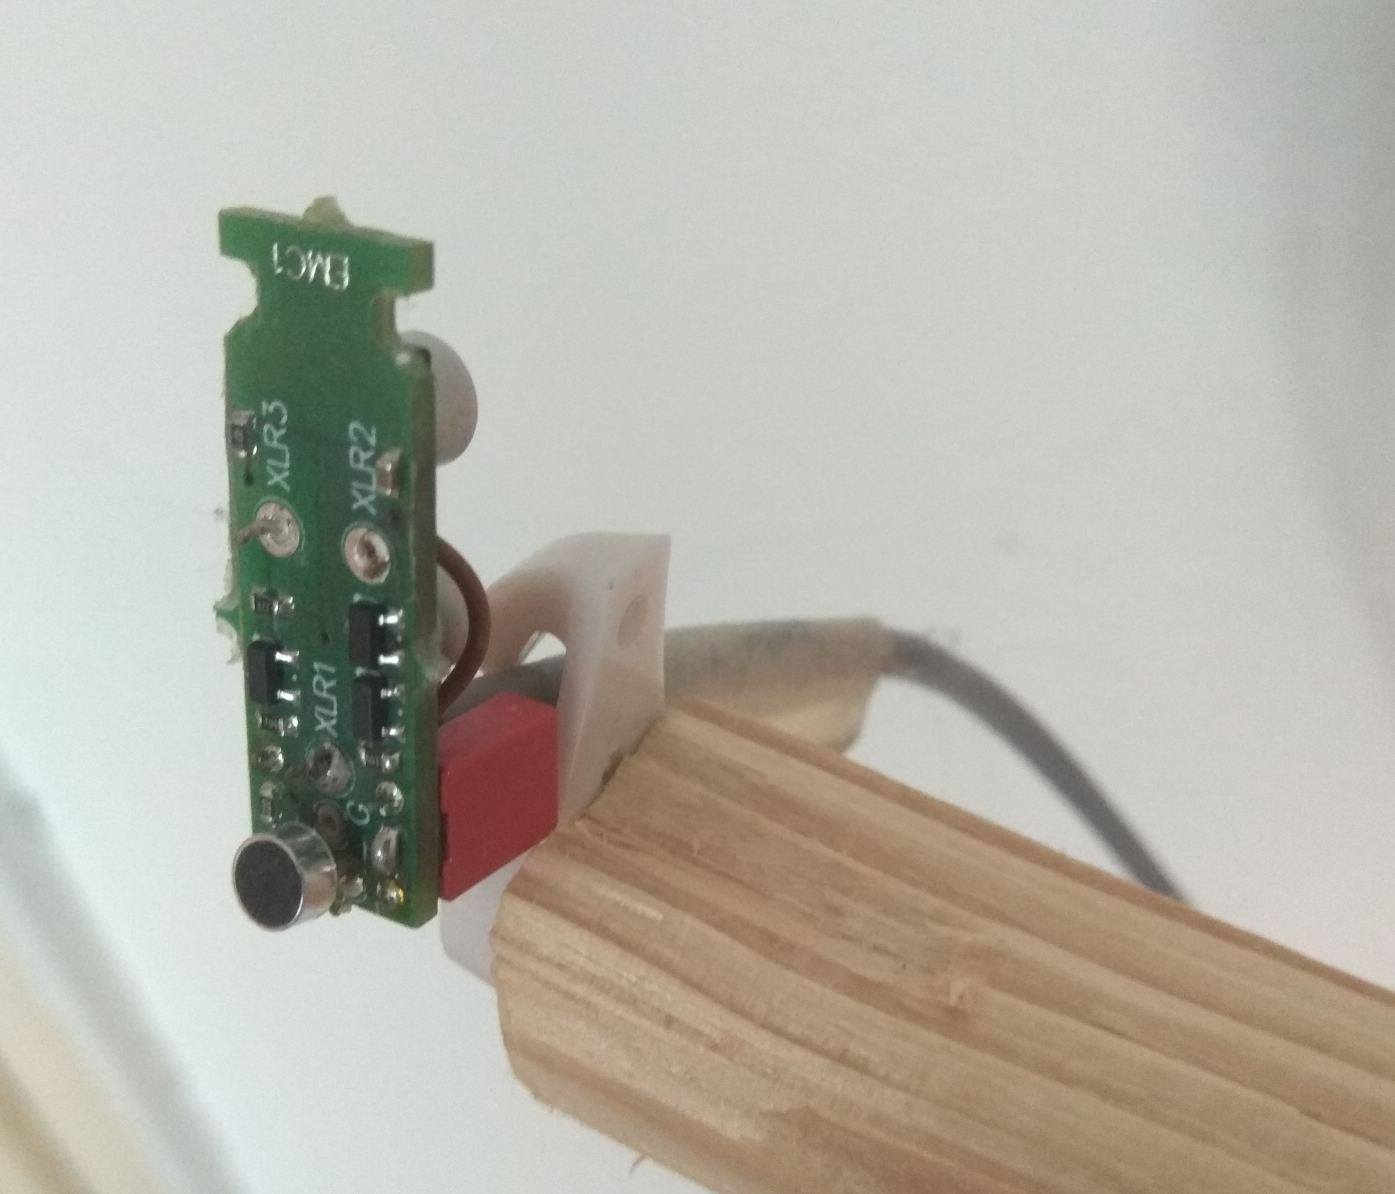
\includegraphics[width=0.7\textwidth]{obrazky-figures/mikrofon_detail.jpg}
	\caption{Detail mikrofonu připevněném na dřevěné konstrukci mikrofonního pole.}
	\label{pic:detail_uchyceni}
\end{figure}

\begin{figure}[!hbt]
	\centering
	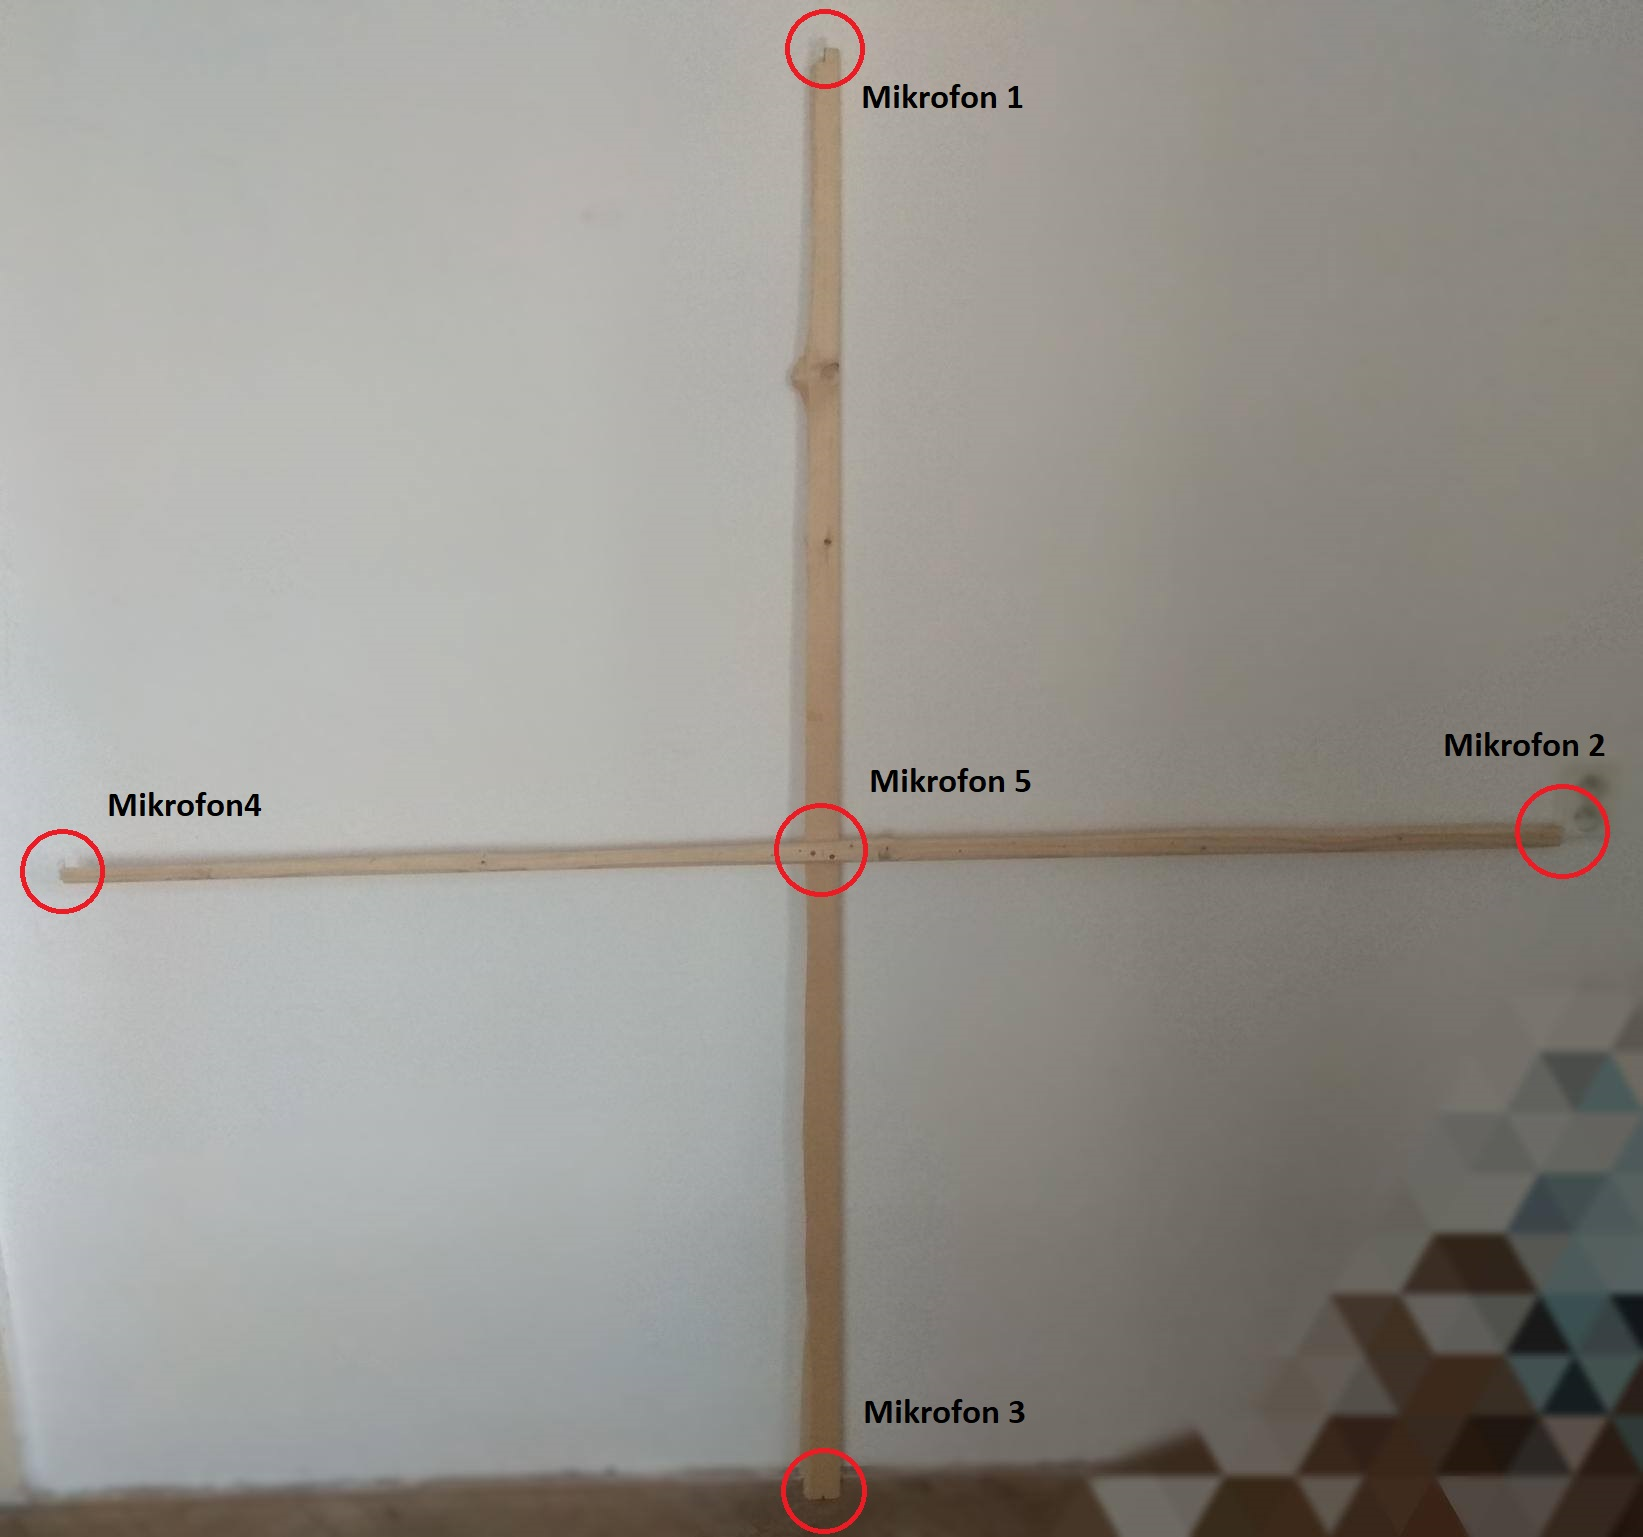
\includegraphics[width=0.7\textwidth]{obrazky-figures/kriz_cely.jpg}
	\caption{Sestavený prototyp mikrofonního pole s~zvukovou kartou (dole) a již některými mikrofony.}
	\label{pic:fotka_krize}
\end{figure}
\newpage
\subsection{Sestava ARM/SHARC}

Pro zpracování dat v~reálném čase mi byla zapůjčena Fakultou informačních technologií VUT v~Brně sestava systému ARM/SHARC (dále jen zvuková karta). Tento hardware byl sestaven společností Audified a je zobrazen na fotografii \ref{pic:zvukovka}. Procesor zvukové karty obsahuje 3 jádra, dvě DSP\footnote{DSP (digital signal proccesing) - digitální signálový procesor. Procesor optimalizovaný pro zpracování signálů.} a jedno ARM\footnote{Architektura procesorů s~redukovanou instruktážní sadou.}. Na DSP jádrech běží veškeré zpracování zvuku z~až šestnácti mikrofonů a ALSA ovladač \cite{alsa}, který využívám ve svém programu. ARM jádro je využito jako výpočetní procesor pro výsledný program. Toto jádro má taktovací frekvenci 450 MHz. Na jádře běží také linuxový systém, který spotřebuje část jeho výkonu. Proto je velmi důležité při úpravách pro zvukovou kartu dbát na optimalizaci, neboť zvuková karta má relativně nízký výkon. 

\begin{figure}[!hbt]
	\centering
	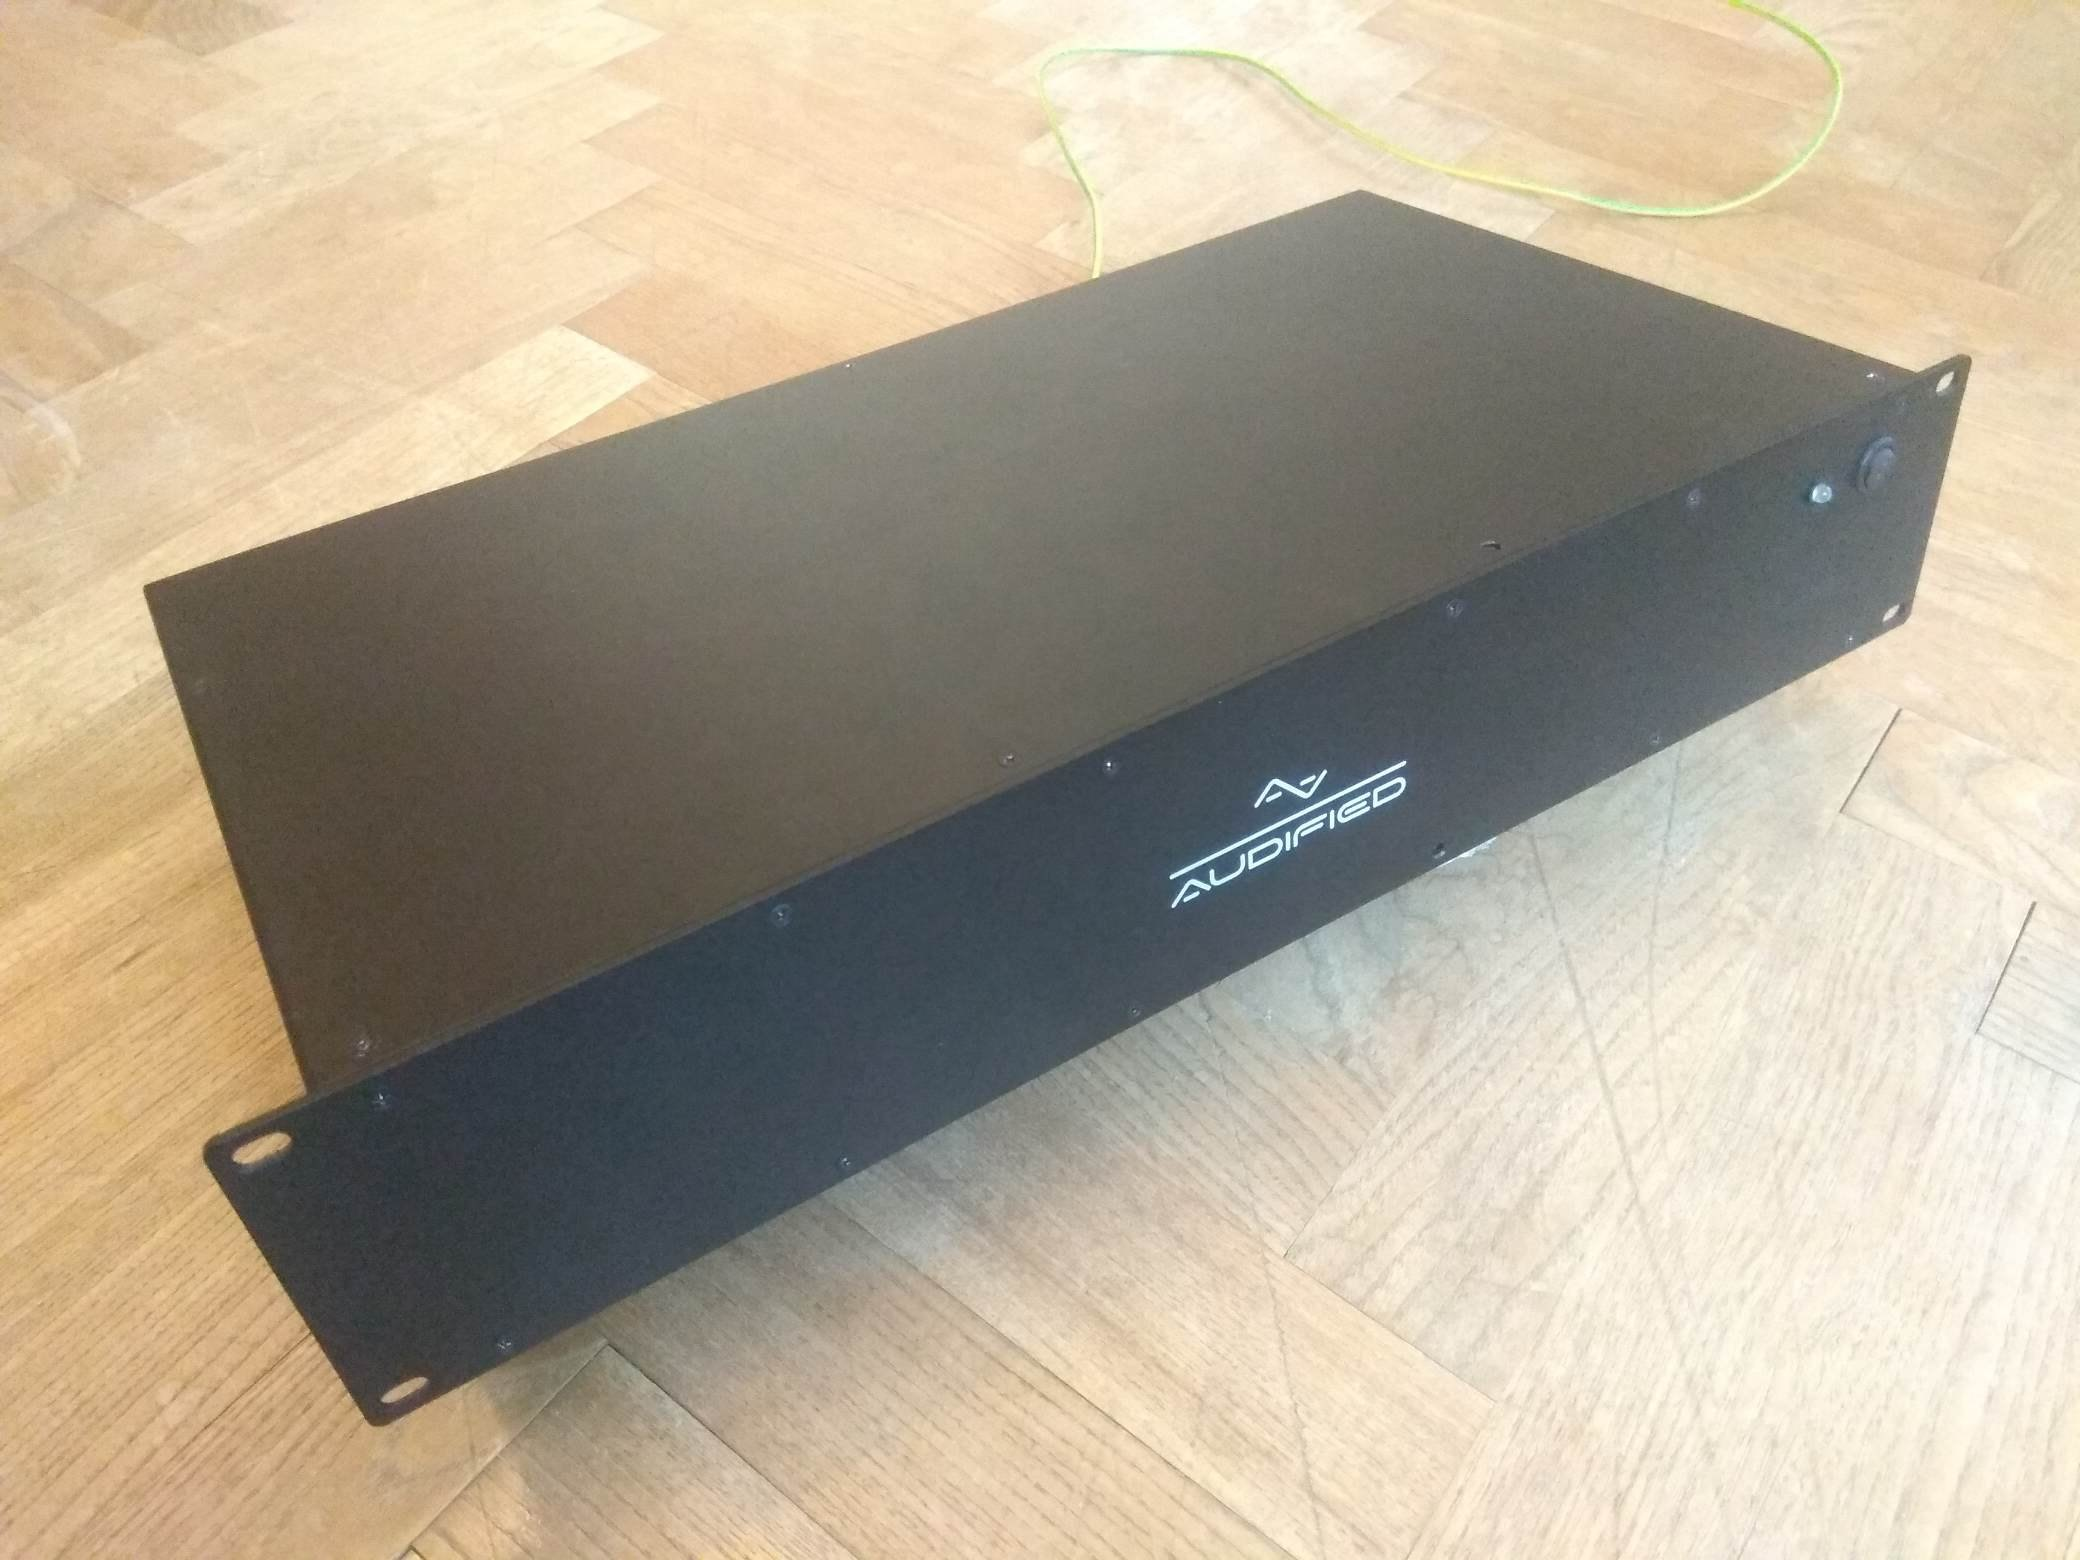
\includegraphics[width=0.6\textwidth]{obrazky-figures/zvukovka.jpg}
	\caption{Sestava ARM/SHARC. Zapůjčena od VUT FIT.}
	\label{pic:zvukovka}
\end{figure}

Zvuková karta obsahuje mimo jiné SD kartu, ethernet připojení a jako paměť má k~dispozici RAM\footnote{RAM (random access memory) - paměť s~přímým přístupem}. Pokud je třeba nahrát data na zvukovou kartu, musí se nahrát dočasně na RAM. Výrobce neumožňuje jednoduše nahrávat data na SD kartu.

Na zvukové kartě není nainstalován překladač, proto pro práci je nutné využití křížového překladače (cross-compiler). Tím lze na jedné platformě přeložit program a vytvořit binární soubor spustitelný na druhé platformě. Poté je možné přes SCP\footnote{SCP - Secure copy (kopírování přes SSH)} nahrát binární soubor přímo do zvukové karty a následně opět přes SSH\footnote{SSH (secure shell) - zabezpečený komunikační protokol} tento soubor spustit. Jak využít vytvořený \texttt{Makefile} a jak pracovat s~programy je popsáno v~souboru \texttt{README} na přiloženém CD.
\newpage
\subsection{Laptop}

Pro testování algoritmů a pro jednodušší úpravy byl využit laptop značky HP ProBook 4740s s~procesorem \emph{Intel(R) Core(TM) i5-3210M CPU @ 2.50GHz, jádra: 2}. Jedno jádro procesoru na laptopu má přibližně pět krát větší taktovací frekvenci než zvuková karta. Je důležité brát také v~úvahu, že laptop má dvě jádra, zatímco na zvukové kartě běží operační systém i zpracování signálu zároveň na jednom jádru.

\section{Implementační řešení bez důrazu na optimalizaci}
\label{navrh implementace}

Nahrávání zvuku, které je znázorněno na schématu \ref{pic:schemanahravani}, je zajištěno mikrofony, které jsou všechny připojené ke zvukové kartě. Karta vytváří synchronizované signály o~vzorkovací frekvenci 48 Khz, které posílá přes webové rozhraní na laptop, kde se ukládají. Tento proces je zajištěn softwarem, který byl dodán se zapůjčenou zvukovou kartou.

\begin{figure}[hbt]
	\centering
	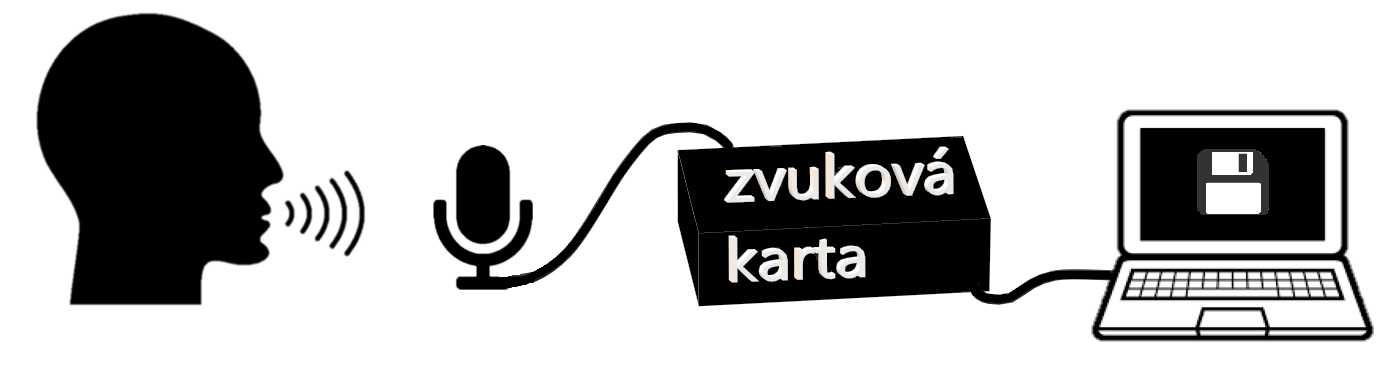
\includegraphics[width=0.9\textwidth]{obrazky-figures/schema_nahravani.png}
	\caption{Řeč je zachycena mikrofony, zpracována zvukovou kartou a uložena na laptopu.}
	\label{pic:schemanahravani}
\end{figure}

Následně program \texttt{voice\_tracker} pracuje s~těmito nahrávkami, jak je znázorněno na schématu \ref{pic:schemantb}.

\begin{figure}[hbt]
	\centering
	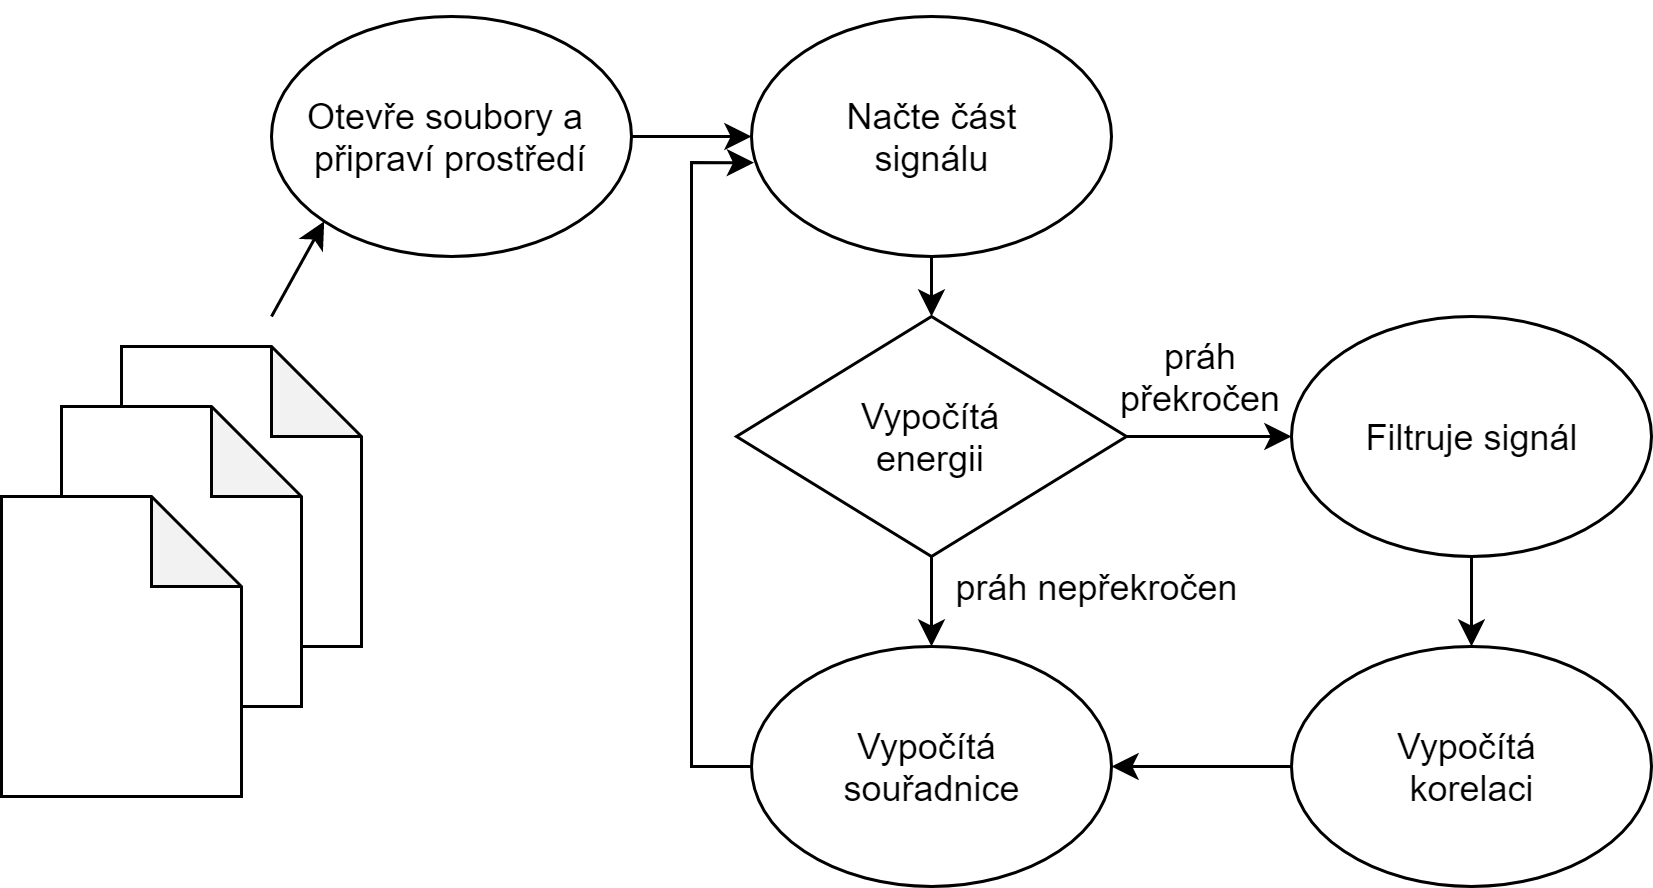
\includegraphics[width=1\textwidth]{obrazky-figures/schema_program.png}
	\caption{Schéma chodu programu na laptopu.}
	\label{pic:schemantb}
\end{figure}

Aplikace \texttt{voice\_tracker} po inicializaci proměnných otevře soubory a načte první část dat tak, abychom měli k~dispozici data z~prostředního mikrofonu s~přesahem 139 vzorků na obě strany pro překrývání při korelaci. Dále pokračuje jeden cyklus, který prochází nahrávky po částech.

V~cyklu se nejprve načtou data ze souborů. Data se načítají po polovinách délky okna signálu. Díky tomu je zajišťen překryv vzorků a je tak dosaženo větší přesnosti. Tento překryv však způsobuje dvojnásobnou výpočetní náročnost.

Dále se počítá součet energií každého zvukového kanálu. Pokud energie přesáhne minimální práh, pokračuje k~výpočtu pozice. Tento práh vychází z~naměřených nejnižších hodnot energie a počítá se jako minimální energie krát prahový koeficient. Pokud je energie nižší než tento práh, snížíme práh na hodnotu vypočtené energie a pokračujeme k~dalším datům. Pokud nižší není, ale zároveň nepřesáhne práh, hodnota prahu se zvýší a program načítá další data v~novém kole cyklu. Postupným zvyšováním minimální energie se zajistí, že prostor může mít různé hladiny hluku okolního hluku v~čase. Může se tak stát, že pokud hluk v~místnosti bude rovnoměrně stoupat nebo například řečník bude mluvit a přicházet z~dálky, tak program nezaregistruje dostatečnou změnu energie, aby jí identifikoval jako zdroj zvuku. Minimální energie se však bude stále zvedat.

\begin{figure}[hbt]
	\centering
	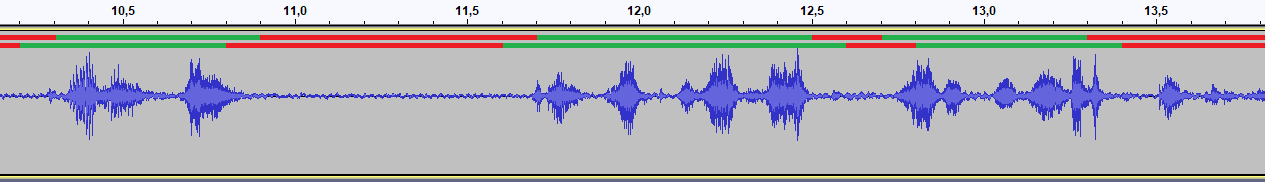
\includegraphics[width=1\textwidth]{obrazky-figures/detekce_hlasu.png}
	\caption{Obrázek ukazuje, jak program detekoval řeč. Červená linie znázorňuje detekované ticho, zelená znázorňuje detekovanou řeč. Dvě linie vyznačují překryv oken.}
	\label{pic:detekce_hlasu}
\end{figure}

Práh byl nastaven na vyšší hodnotu z~důvodu eliminace výpočtů s~šumem. Pokud by byl práh nižší hodnoty, docházelo by ke špatnému výsledku korelace. Pokud by byl práh vyšší hodnoty, docházelo by k~nesprávné detekci hlasu.

Jako další krok je filtrace signálů, která je implementovaná podle vzorce v~sekci \ref{filt}. Je možné vybrat možnost filtrování, a to dolní propusť, pásmová propusť nebo pokračovat bez filtrace. Později jsou testovány důsledky filtrování v~sekci \ref{testfilt}.

Dalším krokem je nejdůležitější, nejnáročnější a nejchybovější část celého programu, korelace. V~programu je možnost zvolit si dvě různé varianty korelace. Buď normalizovanou křížovou korelaci nebo korelaci odečítáním signálů. Zjištění posunu však není nutné dělat po celé délce okna signálů. Víme, jak vzdálené jsou mikrofony od sebe, a tudíž dokážeme spočítat, jaký je nejvyšší možný posun. Hyperbola je počítána mezi mikrofony, které jsou od sebe jeden metr a nejvyšší možné zpoždění je, pokud zdroj zvuku leží na přímce tvořené těmito mikrofony, jako je na obrázku \ref{pic:posun}. Zpoždění se může počítat v~časových jednotkách, nebo při korelaci počítáme bez jednotek, tedy v~počtu vzorků. Zpoždění se vypočítá ze vzdálenosti dvou mikrofonů následovně:

\begin{align}
    \label{eq:maxposun}
    \Delta_f&=(\frac{s}{v_s})f_s, \\
    \Delta_f&=(\frac{1}{343})48000=139,94,
\end{align}

kde $\Delta_f$ je posun, $s$ je vzdálenost mikrofonů a $f_s$ je vzorkovací frekvence.

\begin{figure}[hbt]
	\centering
	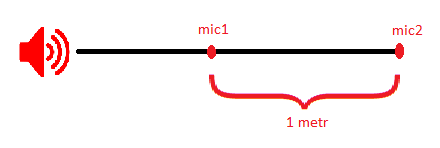
\includegraphics[width=0.6\textwidth]{obrazky-figures/maxRozdil_mikrofonu.png}
	\caption{Případ pozice zdroje zvuku s~maximálním možným zpožděním signálů mezi dvěma mikrofony.}
	\label{pic:posun}
\end{figure}

Maximální posun 139,94 se zaokrouhlí dolů. Posun o~140 vzorků může nastat pouze za určitých podmínek, jako například jiná teplota, jiná hustota vzduchu (jiná rychlost zvuku) nebo nepřesně usazené mikrofony v~poli. Při snížení maximálního posunu se snižuje výpočetní úhel v~prostoru před mikrofonním polem. V~rámci použitelnosti práce si však můžeme dovolit zmenšit výpočetní úhel, protože zdroj se pravděpodobně nebude nacházet příliš blízko roviny, na které leží mikrofonní pole. Dalším důvodem je, že ani analytické řešení nedokáže vypočítat přesnou polohu na takto krajních úhlech. Proč analytické řešení nedokáže vypočítat přesnou polohu blízko roviny mikrofonního pole je vidět na grafech \ref{pic:graf48} a \ref{pic:graf8}, které vykreslují veškeré možné vypočtené pozice zdroje.

\begin{figure}[!hbt]
	\centering
	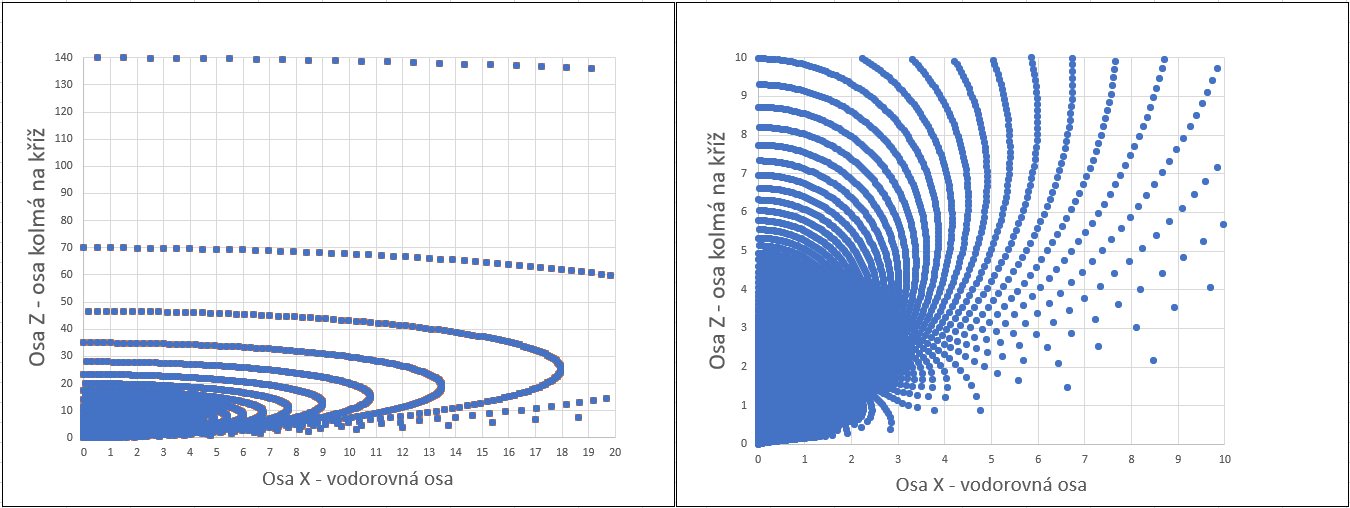
\includegraphics[width=1\textwidth]{obrazky-figures/graf_48khz.png}
	\caption{Na grafu vlevo je většina poloviny výpočetního prostoru. Okno na většinu bodů na souměrné jedné polovině výpočtové plochy. Vpravo přiblížené toto okno na relevantní prostor. Vzorkovací frekvence 48 kHz.}
	\label{pic:graf48}
\end{figure}

\begin{figure}[hbt]
	\centering
	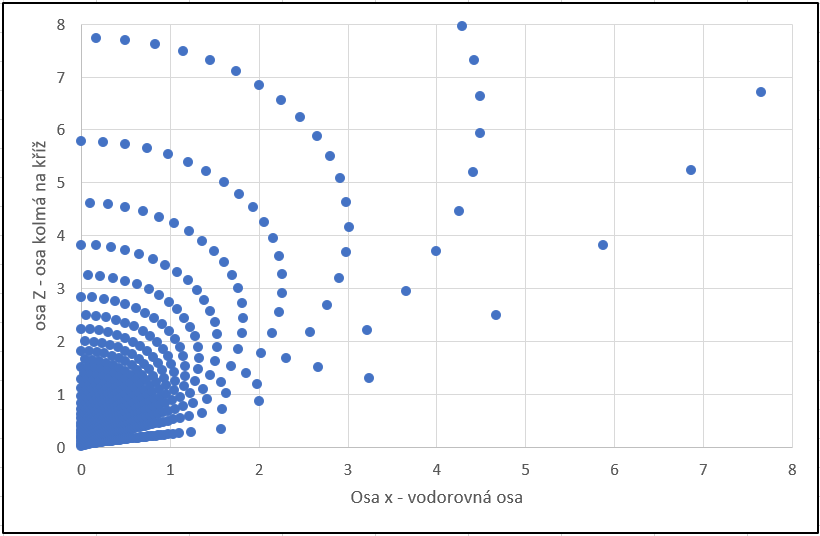
\includegraphics[width=0.8\textwidth]{obrazky-figures/graf_8khz.png}
	\caption{Okno většiny bodů na souměrné polovině výpočtové plochy, při vzorkovací frekvenci 8 kHz.}
	\label{pic:graf8}
\end{figure}

Nyní když známe posun signálů, můžeme vypočítat souřadnice polohy signálů. Pro výpočet polohy musíme zjistit průnik 3 hyperbolických rovin. Tento relativně složitý problém však lze zjednodušit. Výpočet je možné rozdělit na dva výpočty pro každou osu. Tím se získá pro každou osu vzdálenost bodu a posunutí na této ose. Tedy na vodorovné ose se zjistí, jak je posunutý na ose $x$ a jak je vzdálený od této osy. Fakticky to je kružnice kolem této osy, jako je znázorněno na obrázku \ref{pic:TDOA2}. To samé můžeme vypočítat pro svislou osu mikrofonního pole a získáme souřadnici na ose $y$ a vzdálenost od této osy obdobně jako na již zmiňovaném obrázku.

Výpočet průniku dvou hyperbol však není triviální problém. Pro rozlišení souřadnic od výpočtů průsečíků označme v~soustavě rovnic \ref{eq:prusecik} $x$ jako posun na ose $p$ a $y$ označme jako vzdálenost od odpovídající osy $v$. Bezprostředně před výpočtem průsečíku nejsou známé proměnné $p$, $v$, $a_1$, $a_2$, $b_1$ a $b_2$. Proměnné $b_1$ a $b_2$ se vypočítají užitím proměnných $a_1$ a $a_2$ pomocí rovnice \ref{eq:vedlejsipoloosa}. Následně po dosazení souřadnic středu, který je znám před spuštěním programu, po vyjádření $b_1$ a $b_2$ pomocí $a_1$, $a_2$ a znalostí excentricity, která je rovna půlce vzdálenosti mezi mikrofony (ohnisky hyperbol) půl metru. Po dosazení získáme následující rovnici:

\begin{align}
    \label{eq:rovnice_prusecik}
    \frac{(p-0.5)^2}{a_{2}^2}-\frac{(v)^2}{(0.25-a_{2}^2)^2}&=1, \\
    \frac{(p+0.5)^2}{a_{1}^2}-\frac{(v)^2}{(0.25-a_{1}^2)^2}&=1.
\end{align}

Z~první rovnice si vyjádříme $v$:

\begin{equation}
    \label{eq:y}
    v = \sqrt{\frac{(\frac{(p-0.5)^2}{a_{2}^2}-1)}{(\frac{1}{4}-a^2)}  }.
\end{equation}

Druhou rovnici nejdříve upravíme:

\begin{equation}
    p^2 + p = (1+\frac{v^2}{\frac{1}{4}-a_{1}^2})a_{1}^2-\frac{1}{4}.
\end{equation}

Do této rovnice dosadíme $v$:

\begin{equation}
    p^2 + p = (1+\frac{\frac{\frac{(p-0.5)^2}{a_{2}^2}-1}{\frac{1}{4}-a^2}}{\frac{1}{4}-a_{1}^2})a_{1}^2-\frac{1}{4}.
\end{equation}

Nyní lze použít nástroj WolframAlpha \footnote{Nástroj WolframAlpha i s~řešenou rovnicí dostupný na \href{https://www.wolframalpha.com/input/?i=\%28\%28\%281\%2B\%28+\%28\%28\%28\%28\%28y-0.5\%29\%5E2\%29\%2F+++++b\%5E2++++\%29-1\%29+++++*\%280.25-++++b\%5E2++++\%29+\%29\%2F\%280.25-++++a\%5E2+++\%29\%29\%29*+++a\%5E2++++\%29-0.25\%29\%3D\%28y\%5E2\%29\%2By}{www.wolframalpha.com} }, který vrátí výsledek:

\begin{equation}
    p = \frac{-4 a_{2}^2 a_{1} + 4 a a_{1}^2 + a_{2} + 3 a_{1}}{2 (a_{2} + a_{1})} ,a_{2} + a_{1} \neq 0, 4 a_{2} a_{1}^2 - a_{2} \neq 0.
    \label{x}
\end{equation}

Užitím rovnice \ref{x} se vypočítají posuny podél os (výsledné souřadnice $x$ a $y$) a dosazením do rovnice \ref{eq:y} vypočítáme vzdálenosti od os. Souřadnici $z$ lze vypočítat pomocí Pythágorovy věty a z~vypočtených hodnot jako je na obrázku \ref{pic:vypocetz} rovnicí:

\begin{equation}
    z_1 = \sqrt{ |(v_2^2)-(p_1^2)| },
\end{equation}

kde $v_2$ je vzdálenost od svislé osy a $p_1$ je posunutí na vodorovné ose.
Respektive:

\begin{equation}
    z_2 = \sqrt{ |(v_1^2)-(p_2^2)| },
\end{equation}

kde $v_1$ je vzdálenost od vodorovné osy a $p_2$ je posunutí na svislé ose.

V~programu je možné tyto rovnice zkombinovat a vypočítat z~nich průměr. To většinou vede k~přesnější souřadnici $z$.

\begin{figure}[h]
	\centering
	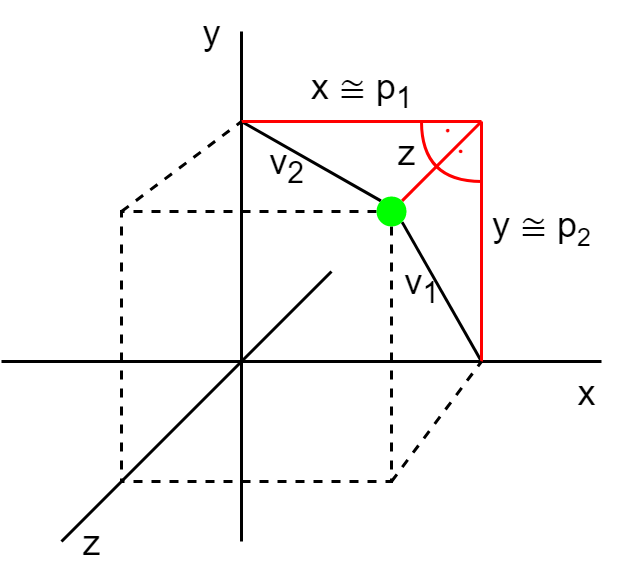
\includegraphics[width=0.5\textwidth]{obrazky-figures/spojeni_x_a_z.png}
	\caption{Vizualizace výpočtu souřadnice $z$. Červeně jsou znázorněny výsledné souřadnice $x$, $y$ a $z$.}
	\label{pic:vypocetz}
\end{figure}

\section{Úprava implementace pro zvukovou kartu}

U~zvukové karty je největší problém její výkon. Pro výpočet v~reálném čase je nutné zajistit, aby tento výpočet trval maximálně stejnou dobu, jako je délka počítaného okna. Jako příklad je uvedeno spuštění normalizované korelace bez použití filtrace a překrývání vzorků. Při výpočtu s~oknem o~délce 0,128 vteřin (6144 rámců) trval přibližně 0.750 vteřiny. Výpočet proto musí být alespoň o~$$0.750-0.128=0.622 s$$ kratší. Je třeba optimalizovat výpočet o~necelých 83 \%.

Možností, jak urychlit proces výpočtu nebo jak pomoci zvukové kartě v~rychlejším výpočtu, je několik. Lze přeskakovat data. Tento způsob by fungoval za předpokladu, že se nebude přeskakovat takové množství dat, aby to narušilo přesnost výpočtu. Nebo-li pokud je jeden výpočet okna špatně, tak výpočet polohy bude minimálně na 0,75 vteřiny chybný. K~chybě může přispět i menší odmlka v~hlase a nepřesnost se může projevit i na několik vteřin.

Možností je výpočet na kratších oknech. Z~okna 6144 rámců (rámec je jeden vzorek z~každého kanálu) můžu počítat například pouze s~první polovinou. Tímto způsobem bohužel mohu zahodit část vzorku, kde se právě nachází řeč a tím znehodnotit celý výpočet. Naštěstí však budu počítat dostatečně často, abych mohl případnou neshodu ihned opravit. Například pokud by se objevila chyba, další výpočet přijde téměř okamžitě a má možnost tuto chybu přehodnotit. Navíc tímto způsobem se nesnižuje kvalita vzorkování což může být velmi důležité pro přesnější výpočet pozice.

Změna vzorkování na nižší vzorkovací frekvenci umožní snížit výpočetní náročnost. Toto se ale projeví na přesnosti výpočtu pozice. To lze vidět na dvou grafech výše. Na grafech \ref{pic:graf48} jsou veškeré vygenerované možné body, které lze získat analytickým výpočtem při vzorkovací frekvenci 48 kHz. Za povšimnutí stojí, že úhel výpočtu nepokryje celých 180\degree \\ a ve větších vzdálenostech dochází ve výpočtu k~nepřesnostem. Pro porovnání graf \ref{pic:graf8} ukazuje veškeré vygenerované body pro vzorkovací frekvenci 8 kHz, kde i při přesné korelaci by na vzdálenosti pěti metrů mohla být chyba až půl metru. Otázka, která nastává je, zda je to dostatečná přesnost.

Pro dostatečné zkrácení výpočtu a neznehodnocení výsledku je třeba využít více těchto možností zkrácení výpočtu. Funkční řešení je snížit vzorkovací frekvenci na například 8 kHz. Tato úprava zvýší nepřesnosti v~určení polohy jako je na grafech \ref{pic:graf48} a \ref{pic:graf8}. Zlepšení přesnosti lze tedy dosáhnout snížením vzorkovací frekvence.

Takovouto úpravu však nemusíme dělat hned při načtení dat, ale můžeme přeskakovat hodnoty jen v~nejnáročnější části programu, tedy korelaci. Korelační metody by při zpracovávání hlasu měly dobře fungovat i při frekvenci 8 kHz. Zároveň nechceme ztratit přesnost, jak je na grafech \ref{pic:graf48} a \ref{pic:graf8} při výpočtu pozice. Proto v~cyklu, kde procházíme pole hodnot ve frekvenci 48 kHz budeme počítat pouze s~každou šestou hodnotou a tím se dostaneme ve výpočtu korelace na vzorkovací frekvenci 8 kHz a snížíme výpočetní náročnost na šestinu. Toto však stále pro zvukovou kartu nestačí a výpočet nestíhá. Využijeme proto možnosti uřezávat části oken a tím zmenšit výpočetní náročnost. Experimentálně bylo vyzkoušeno zkracovat okno o~1270 rámců. I~v~tomto případě zvuková karta občas nestihla výpočet z~důvodu nutnosti dělit se o~jádro se systémem a jinými aplikacemi. Proto jsem vzorek zmenšil o~1300 rámců a tím zajistil nepřerušovaný průběh programu. Níže je uveden zjednodušený příklad, jak tato úprava může vypadat v~kódu.

\begin{lstlisting}[language=C]
// pro každý posun od -139 do +139 (279)
for(int i = 0; i < 279 ; i++)       
{
        // projde v~okně pouze každou šestou hodnotu – zkrátí toto okno o~N vzorků
	for(int j = 0;j<SAMPLE_LEN-N;j+=6)      
	{	
		// zde se provede korelace (suma kartézského součinu)
	}
    // zde se zapíše výsledek do pole statistik
}
\end{lstlisting}

\chapter{Testování komponent programu}
\label{testovani}

Testování probíhalo v~místnosti přibližně 6x5 metrů. Nahrávky vznikaly přehráváním stejného záznamu z~mobilu. Jako testování reálných dat proběhly i testy s~reálným slovním projevem člověka bez použití reproduktoru. Byly provedeny testy detekce řeči a ideálního prahového koeficientu, testy výpočtu polohy, pokusy s~filtrováním signálu a otestování vhodnější korelační metody.

\section{Test výpočtu energie}

Pomocí výpočtu energie se zajišťuje filtr šumu. Pokud se dokáže správně určit část s~řečí, pak se můžou určit i místa s~šumem. Důležitý aspekt tohoto výpočtu je, aby se nestalo, že se bude počítat s~velmi tichou řečí, případně dokonce jen s~šumem. Proto bylo důležité určit správně koeficient energetického prahu, kterým se dá dobře určit, kde je možné vypočítat korelaci a kde by výpočet mohl mít velké odchylky.

Test probíhal zpracováním nahrávky a následným porovnáním vizualizace signálu a poslechem signálu. Z~vizualizace nejlépe vychází prahový koeficient 2,5. Je třeba mít na zřeteli, že toto stanovení koeficientu prahu je závislé na citlivosti mikrofonu a hlasitosti zdroje zvuku.

Výše na obrázku \ref{pic:detekce_hlasu} je už takové testování znázorněné s~překryvem oken při použití délky okna 9600 rámců. Na dalších obrázcích je znázorněná detekce bez překryvu oken s~různými prahovými koeficienty a s~délkou okna 6144 rámců, tak jak později běží na zvukové kartě. Nahrávka je spuštěna mobilním telefonem 1 metr vzdáleným od mikrofonu.

Při porovnání lze vidět, že nejnižší práh 2 funguje dobře právě například při odfiltrování šumu, bohužel ale zabírá velkou část ozvěn a jiných menších rušení signálu. Tento práh by byl použitelný, ale zvyšoval by nepřesnost výpočtu korelace. Naproti tomu nejvyšší práh 4 lokalizuje jen velké amplitudové výkyvy. Proto by mohl být využit pro zpřesnění korelace, která by počítala jen s~výraznými signály a byla by větší jistota, že nejde o~ozvěnu nebo rušivý zvuk. Tím, že ale počítá s~vysokou intenzitou zvuku nelze detekovat tichý zdroj zvuku.

\begin{figure}[ht]
	\centering
	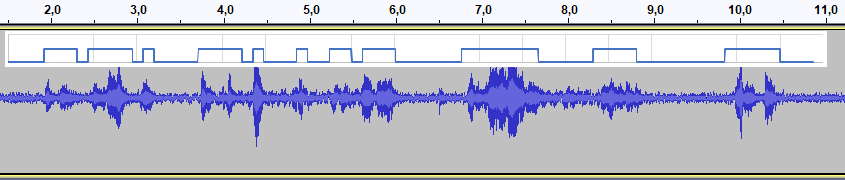
\includegraphics[width=1\textwidth]{obrazky-figures/energy2.png}
	\caption{Detekovaný hlas při prahovém koeficientu 2.}
\end{figure}

\begin{figure}[ht]
	\centering
	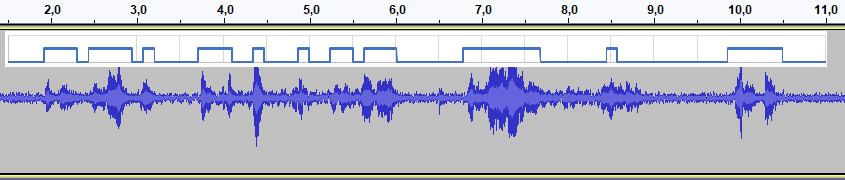
\includegraphics[width=1\textwidth]{obrazky-figures/energy25.png}
	\caption{Detekovaný hlas při prahovém koeficientu 2,5.}
\end{figure}

\begin{figure}[!ht]
	\centering
	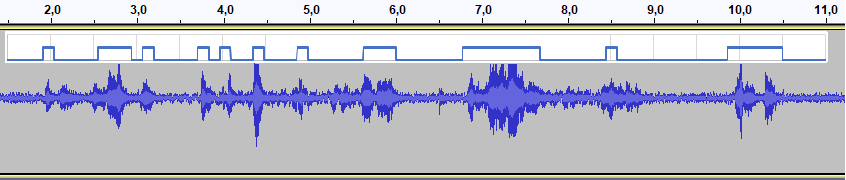
\includegraphics[width=1\textwidth]{obrazky-figures/energy3.png}
	\caption{Detekovaný hlas při prahovém koeficientu 3.}
	\label{pic:ene3}
\end{figure}

\begin{figure}[!ht]
	\centering
	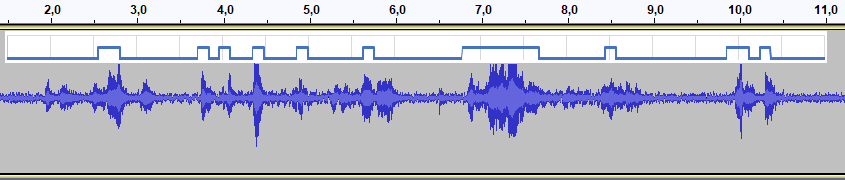
\includegraphics[width=1\textwidth]{obrazky-figures/energy4.png}
	\caption{Detekovaný hlas při prahovém koeficientu 4.}
\end{figure}
\newpage
\section{Test výpočtu polohy analytickým řešením}

Analytický výpočet polohy je funkce, která má jasně daný vstup. Tedy ze čtyř zpoždění signálů z~krajních mikrofonů vůči signálu z~prostředního referenčního mikrofonu se vypočítají souřadnice. Tím se testování zjednodušuje, protože víme, že do funkce nemohou přijít jiné hodnoty, než v~intervalu od -139 do +139. Program \texttt{coor.c} byl vytvořen pouze za účelem testu tohoto výpočtu. Obsahuje funkci na generování všech možných bodů, které bylo využito pro vytvoření grafů \ref{pic:graf48} a \ref{pic:graf8}. Hlavní účel však měl pro zpětný výpočet. Tento výpočet probíhal tak, že zadané souřadnice nejdřív převedl na zpoždění signálů z~mikrofonů, tato zpoždění zaokrouhlil na celá čísla z~důvodu práce s~diskrétními signály a následně zavolal stejnou funkci, která se používá v~hlavním programu \texttt{voice\_tracker}.

Tohoto způsobu zpětného výpočtu bylo využito na zjištění minimální, maximální a průměrné chyby v~pomyslné krychli kolem zadaného bodu. Tedy pro každý $cm^3$ bylo vypočítáno, kde by se tento bod následně objevil. V~tabulce \ref{tabulka} lze vidět některé zajímavé body. Je zde zaznamenán záznam celého prostoru místnosti, ve které byla většina experimentů prováděna.

\begin{table}[!h]
    \centering
    \begin{tabular}{||l | c | c | c||} 
 \hline
 bod & minimum (cm) & maximum (cm) & průměr (cm) \\ [0.5ex] 
 \hline\hline
 [0,0,2] & 0,01 & 5,03 & 1,03 \\ 
 \hline
 [0,0,10] & 0,03 & 75,48 & 18,08 \\
 \hline
 [2,2,2] & 0,03 & 18,86 & 4,69 \\
 \hline
 [3,1,5] & 0,02 & 35,34 & 9,26 \\
 \hline
 [5,1,1] & 0,26 & 729,62 & 138,64 \\
 \hline
 [15,15,50] & 400,79 & 1211,22 & 760,99 \\
 \hline
 místnost & 0,00 & 337,6 & 5,36 \\ [1ex] 
 \hline
    \end{tabular}
    \caption{Chyby při výpočtu polohy zdroje zvuku analytickým řešením při nutnosti zaokrouhlovat zpoždění.}
    \label{tabulka}
\end{table}


Je možné pozorovat podobnost větších nepřesností s~podobnými místy na grafu \ref{pic:graf48}.

\section{Test filtrování}
\label{testfilt}
Filtrovat by se ideálně měly frekvence odpovídající lidskému hlasu. Ze sekce \ref{hlas a sluch} je zřejmé, že hlas má frekvence do 10 kHz a frekvence nutné k~porozumění nepřesahují 3 kHz. Hlas však obsahuje neharmonické složky, proto filtrování nemusí nutně mít zásadní vliv na výsledky výpočtů korelace. Základní složky hlasu jsou v~rozsahu 100 Hz až 3 kHz \footnote{základní složky lidského hlasu na stránce \href{https://www.seaindia.in/human-voice-frequency-range/}{www.seaindia.in}}, proto byla zvolena horní propusť na 3 kHz a dolní propusť na 100 Hz. Na obrázcích můžete vidět, jak byly filtrovány dva signály obsahující nejběžnější složku komorní $A$ (440 Hz) a jednu rušivou složku 50 Hz \ref{pic:HPF} respektive 5000 Hz \ref{pic:LPF}. Dále na obrázku \ref{pic:BPF} je ukázka filtrování jedné z~nahrávek.

Z~obrázků je jasné, že filtr nedokáže odfiltrovat ani frekvence 2x rozdílnější než zadané mezní frekvence. Je proto možné nastavit užší pásmo filtrování nebo použít jiné filtry, které mají strmější charakteristiku.

\begin{figure}[h]
	\centering
	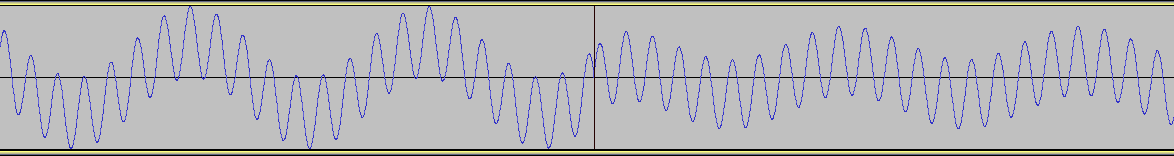
\includegraphics[width=1\textwidth]{obrazky-figures/filtHPF.png}
	\caption{Na levé polovině obrázku nefiltrovaný signál frekvence 50 Hz a 440 Hz, na pravé straně filtrovaný tento signál.}
	\label{pic:HPF}
\end{figure}

\begin{figure}[!h]
	\centering
	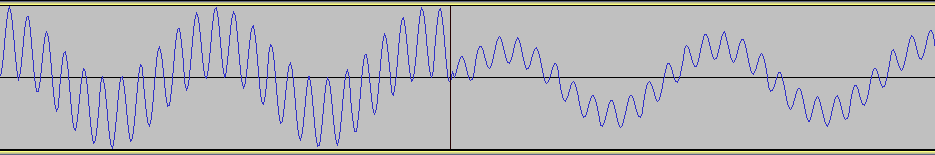
\includegraphics[width=1\textwidth]{obrazky-figures/filtLPF.png}
	\caption{Na levé polovině obrázku nefiltrovaný signál frekvence 5000 Hz a 440 Hz, na pravé straně filtrovaný signál.}
	\label{pic:LPF}
\end{figure}

\begin{figure}[!h]
	\centering
	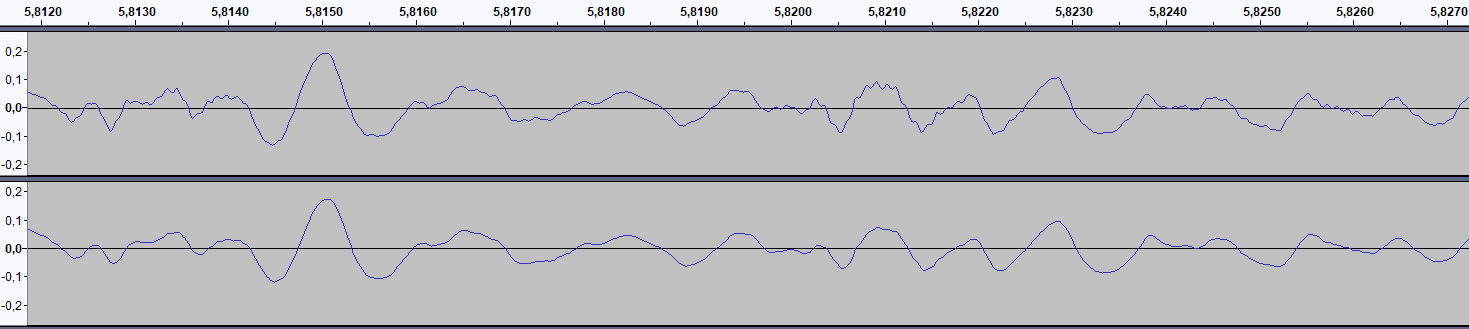
\includegraphics[width=1\textwidth]{obrazky-figures/filtRec.png}
	\caption{Nahoře obrázku je nefiltrovaná část signálu s~řečí. Dole je filtrovaný signál.}
	\label{pic:BPF}
\end{figure}

\newpage
V~tabulce \ref{tabulka5} je znázorněn vliv filtrace signálů na určení polohy zdroje zvuku. Z~výsledku není jasné zda má filtrace kladný vliv na výsledky. Z~experimentů se zdá, že výsledky spíše zhoršuje. Z~toho důvodu a také kvůli rychlosti výpočtu nebyla filtrace později využita.

\begin{table}[!h]
    \centering
    \begin{tabular}{|| l | l | c | c||} 
 \hline
 typ testu & Těžiště bodů & odchylka těžiště & body v~toleranci \\ [0.5ex]
 \hline
 test na [0,0,3] bez filtru & [-0,308; 0,067; 2,958] & 0,318 & 78,9 \% \\ 
 \hline
 test na [0,0,3] s~LPF & [-0,335;-0,161; 2,815] & 0,415 & 87,7 \% \\
 \hline
 test na [0,0,3] s~BPF & [-0,297; 0,093; 2,825] & 0,357 & 73,2 \% \\
 \hline
 test na [1,0,3] bez filtru & [ 0,610; 0,142; 2,626] & 0,558 & 64,5 \% \\
 \hline
 test na [1,0,3] s~LPF & [ 0,506; 0,220; 2,263] & 0,913 & 27,3 \% \\
 \hline
 test na [1,0,3] s~BPF & [ 0,607; 0,543; 2,188] & 1,052 & 25,9 \% \\
 \hline
 test na [1,0,4] bez filtru & [ 0,147; 0,117; 3,525] & 0,983 & 36,5 \% \\ 
 \hline
 test na [1,0,4] s~LPF & [ 0,194; 0,080; 3,523] & 0,939 & 40,2 \% \\
 \hline
 test na [1,0,4] s~BPF & [ 0,243; 0,156; 3,545] & 0,896 & 45,8 \% \\ 
 \hline
    \end{tabular}
    \caption{Porovnaní vlivu filtrace signálu na určení polohy statického zdroje zvuku. V~tabulce je uvedeno těžiště všech vypočtených bodů, odchylka těžiště od správného bodu a počet bodů v~tolerované odchylce maximálně 0,5 metrů.}
    \label{tabulka5}
\end{table}

\section{Test korelačních metod}

Testování korelace proběhlo na generované funkci sinus. Generovaná funkce sinus byla rušena bílým šumem (white noise). Pokud uvažujeme, v~jaké situaci počítáme korelaci, tedy že energie počítaného okna je 2,5krát vyšší než minimální energie ostatních oken, pak můžeme testovat korelaci v~mírně horších podmínkách. Tedy situaci, kdy energie vzorku signálu s~šumem bude dva krát větší než energie pouhého šumu, neboli SNR\footnote{SNR (signal to noise ratio) – poměr signálu ku šumu} je rovné 1. Obě metody, normalizovaná křížová korelace i korelace odečítáním, však dopadli velmi dobře a dokázali správně určit posun i přes prostorový aliasing \ref{pic:SNR1}. 

Z~tohoto důvodu byly podmínky záměrně zhoršeny na SNR 0,162 při kterých již docházelo ke špatnému určení korelace a byla tedy možnost vybrat kvalitnější metodu. SNR 0,162 odpovídá šumu o~amplitudě 0,5 a signálu na dvou třetinách délky okna o~amplitudě 0,2. Vizualizace takového signálu je na obrázku \ref{pic:signalSNR01}. Na grafech \ref{pic:SNR01} je znázorněna četnost posunů, které korelační metody vypočítaly jako maximální. Při správném posunu o~-50 normovaná křížová korelace určila výsledek v~intervalu -40 až -60 ve 48,8 \% případů a korelace odečítáním ve 44,9 \% případů. Můžeme tedy říct, že normovaná křížová korelace dává lepší výsledky, proto byla využita jak pro zvukovou kartu, tak i pro experimenty.

\begin{figure}[hbt]
	\centering
	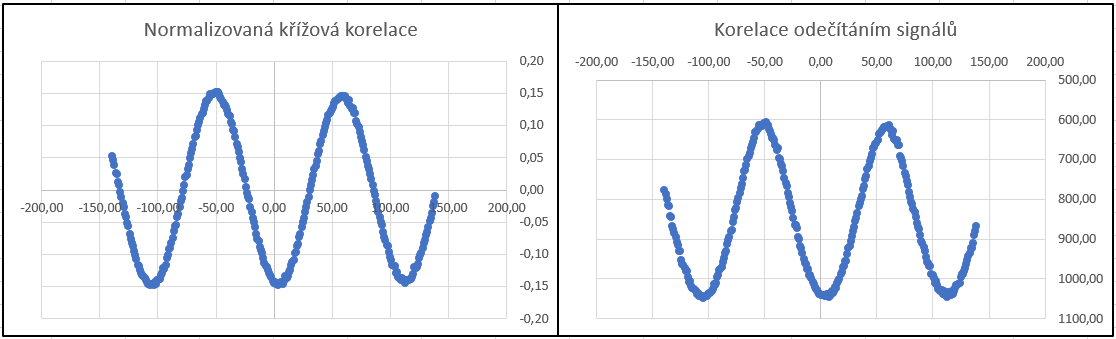
\includegraphics[width=1\textwidth]{obrazky-figures/korelSNR1.png}
	\caption{Grafy ukazují vypočítanou korelaci pro zašuměnou generovanou funkci sinus. Je také vidět jak vypadá vliv aliasingu - více lokálních maxim.}
	\label{pic:SNR1}
\end{figure}

\begin{figure}[hbt]
	\centering
	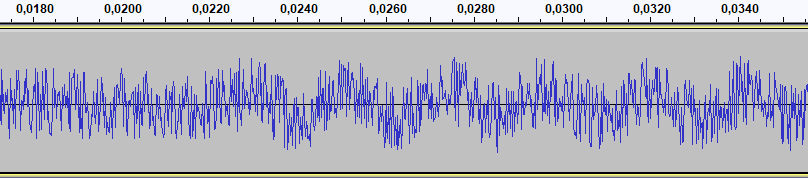
\includegraphics[width=1\textwidth]{obrazky-figures/signal_SNR016.png}
	\caption{Vizuální ukázka signálu při SNR 0,162.}
	\label{pic:signalSNR01}
\end{figure}

\begin{figure}[hbt]
	\centering
	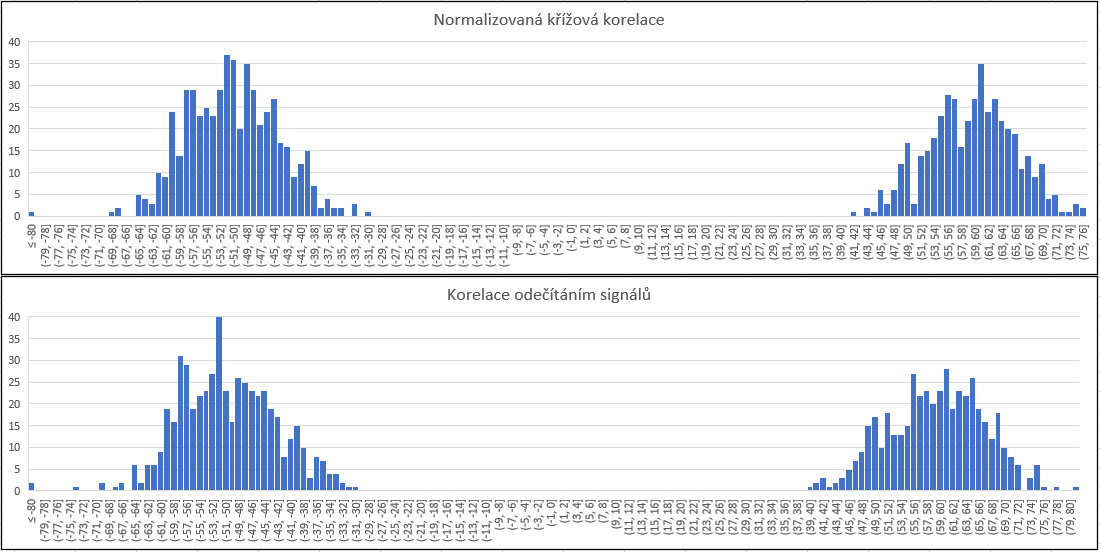
\includegraphics[width=1\textwidth]{obrazky-figures/korelSNR01.png}
	\caption{Grafy ukazují četnost jednotlivých maximálních hodnot z~velmi zašuměného signálu při SNR 0,162 u~dvou korelačních metod.}
	\label{pic:SNR01}
\end{figure}

\chapter{Experimentální výpočty na reálných datech}
\label{experimenty}

V~této kapitole je popsán postup vytváření experimentů od začátků až po testování na zvukové kartě. Jsou zde rozebrány vlivy koeficientů prahu, filtrování a délky okna na reálných datech. Popsány možné vlivy na nepřesnosti korelací. A~nakonec je vyhodnocena nejlepší kombinace.

Pro verifikaci systému je nutné určit metriku, jak lze určit chybovost systému. Při detekci pozice řečníka můžeme tolerovat prostor okolo určení polohy z~pohledu na velikosti řečníka a také z~pohledu na možné nepřesnosti při umístění testovacího zdroje zvuku. Tento prostor je zvolen na půl metru v~okolí zdroje. Pro zjednodušení zobrazení bodu je uváděn pouze půdorys, tedy souřadnice $x$ a $z$. Výpočty však probíhaly včetně osy $y$ v~3D prostoru. 

\section{Nahrávání v~nezatlumené místnosti}

Počáteční experimenty sloužily jako nahrávky pro experimenty v~prvotní fázi vývoje. Nebylo dokonale dbáno na rozmístění mikrofonů a na přesnou polohu zdroje. Sloužily hlavně jako testování elementární funkčnosti programu.

Byla vytvořena desetivteřinová nahrávka mluveného slova, která byla využita i později. Nahrávka se skládala pouze z~mužského hlasu. Tato nahrávka byla spouštěna z~několika míst před mikrofony, jako je na obrázku \ref{pic:testovacipripady}.

\begin{figure}[!ht]
	\centering
	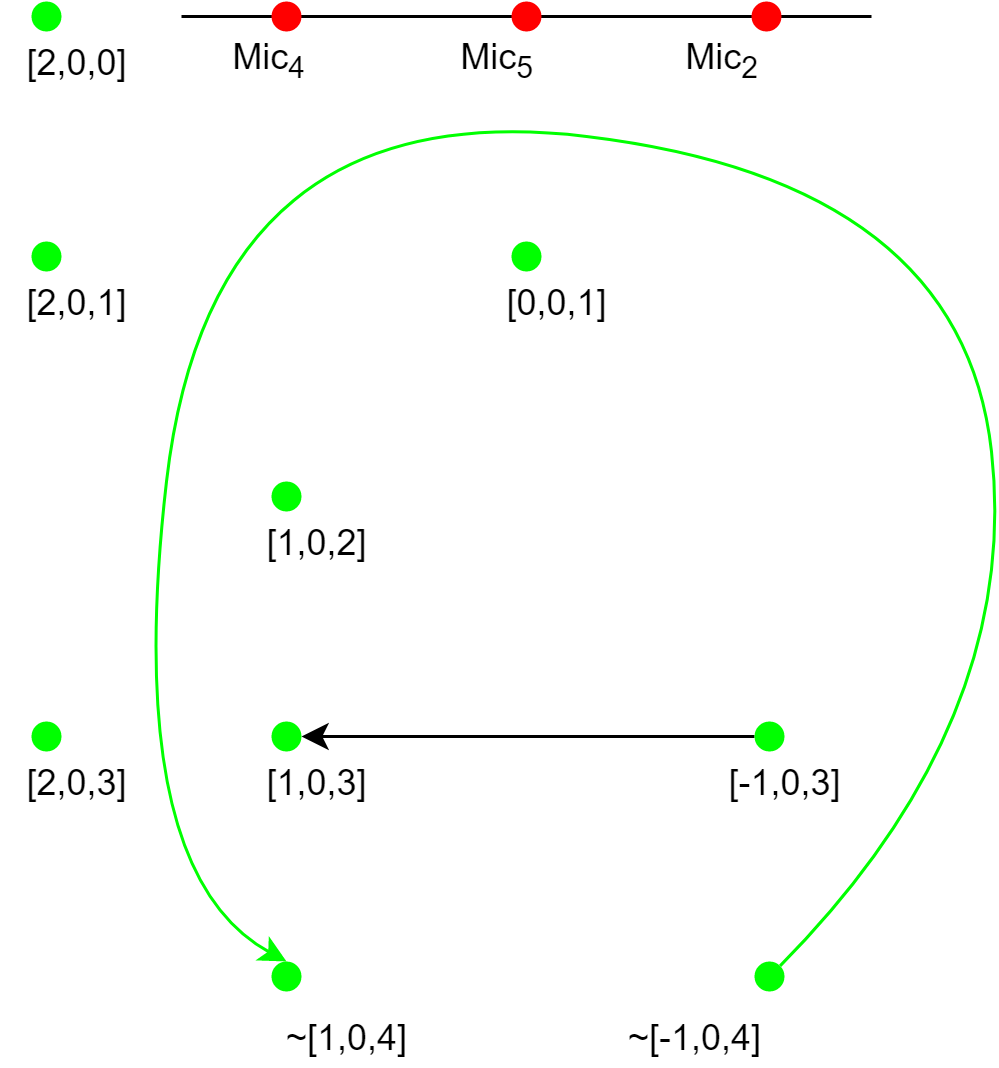
\includegraphics[width=0.5\textwidth]{obrazky-figures/testovaci_pripady.png}
	\caption{Nahrané testovací případy při prvním nahrávání. Pohled shora.}
	\label{pic:testovacipripady}
\end{figure}

Testování na těchto datech se však ukázalo problémové. Jako příklad můžeme uvést test na souřadnicích [0,0,1] a [0,0,3] \ref{pic:test1}. Při experimentování blízkého zdroje byla chybovost velmi malá 29 \%. Tato chybovost byla navíc způsobená převážně prvními dvěma vteřinami nahrávky. Pokud bychom ignorovali první 2 vteřiny byla by chybovost 6 \%. Oproti tomu zdroj zvuku 3 metry vzdálený měl chybovost 98 \%. Je jasné, že další experimenty byly odloženy a bylo nutné najít příčinu.

\begin{figure}[!ht]
	\centering
	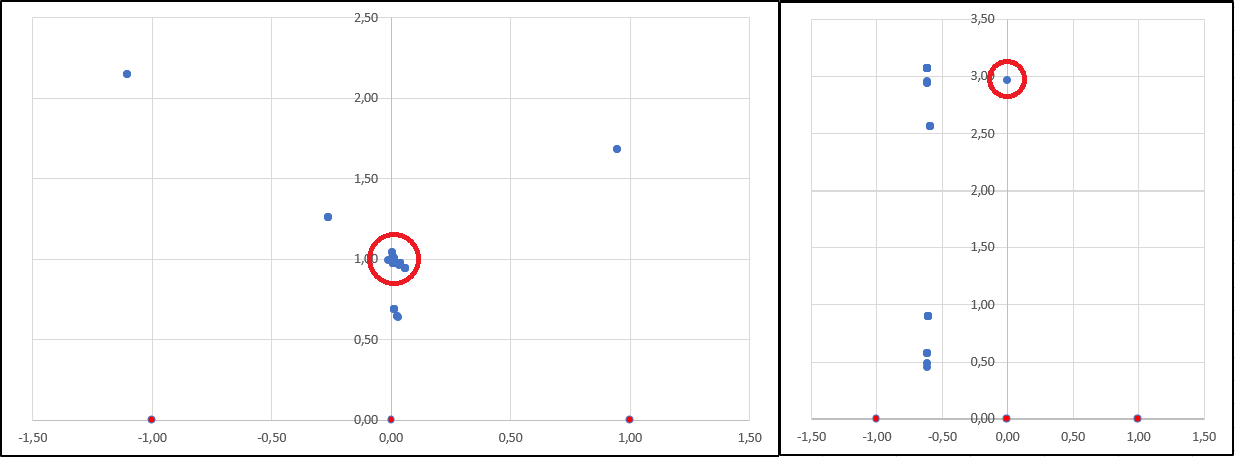
\includegraphics[width=1\textwidth]{obrazky-figures/graf_nezatlumene.png}
	\caption{Testy nahrávek v~nezatlumené místnosti. Vlevo test na souřadnicích [0,0,1] a vpravo na [0,0,3].}
	\label{pic:test1}
\end{figure}

\section{Vlivy na přesnost korelace a celkového výpočtu}
\label{vlivy}

Důležité pro zlepšení výsledků je určit příčinu chybovosti a následně ji potlačit. V~této sekci jsou jednotlivé možné příčiny popsány a rozebrány. Je uvedeno možné řešení a u~vlivů, u~kterých je to možné, jsou uvedena data na základě kterých, se dá rozhodnout, zda je nutné je řešit.

\subsection{Ozvěna}

Ozvěnu jsem zařadil na první místo. Jediný způsob, jak změřit vliv dozvuku na výsledky měření je nahrát signál v~nezatlumené místnosti a následně zkusit zatlumit místnost a opakovat co nejpodobnější test znovu. Spuštění se stejnými parametry lze vidět na grafech \ref{pic:test2}. Rozdíl v~chybovosti je obrovský vzhledem k~tomu, že vznikne pouhou ozvěnou v~pokoji. Test proběhl na stejném místě pouze s~přidáním tlumících prvků jako je na fotografii \ref{pic:neporadek}.

\begin{figure}[hbt]
	\centering
	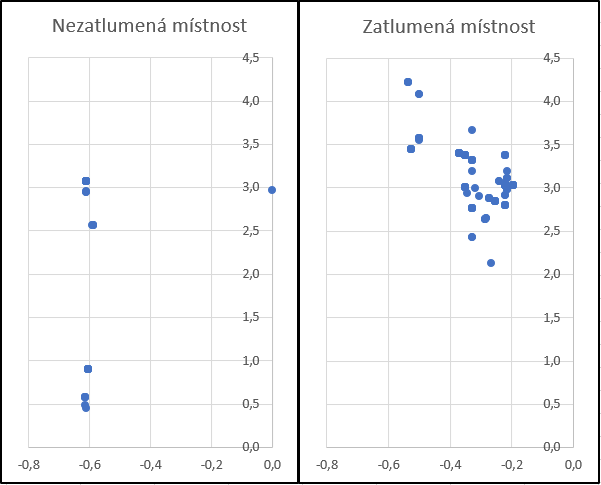
\includegraphics[width=0.6\textwidth]{obrazky-figures/graf_zatlumeneVSnezatlumene.png}
	\caption{Graf ukazuje vlevo nahrávání v~nezatlumené místnosti a vpravo v~zatlumené místnosti. Energetický práh byl nastaven na 3, okno bylo dlouhé 6144 rámců a signál nebyl filtrován. V~prostoru 1x1 metr kolem zdroje bylo v~nezatlumené místnosti 1,6 \% výsledků a v~zatlumené místnosti 90,5 \%.}
	\label{pic:test2}
\end{figure}

Dozvuku se nikdy nedá zbavit úplně, může se však velmi snížit jeho vliv na určení pozice zvuku. Jako příklad můžeme uvést, že podle zdroje \cite{odrazy} se odráží od omítnuté zdi 97,5 \% signálu, od dřevěné podlahy je to 90 \% a například od koberce 71 \%. Ozvěna byla potlačena různými dekami, peřinami a věšákem s~oblečením jak je vidět na fotografii \ref{pic:neporadek}. Běžná praxe zlepšování akustiky prostoru jsou koberce na podlahách a zdech. Pro lepší výsledky pomůže i otevřené okno, protože ruch z~ulice má na výsledky menší vliv než ozvěna signálu, který se snažíme korelovat.

Dále se může snížit dopad ozvěny na výslednou pozici zdroje přidáním prahu korelačního koeficientu. Tento koeficient odpovídá výsledku vypočtené korelace. Přidáním prahu bychom zajistili výpočet s~korelací pouze tehdy, když bychom si mohli být jistí nezkreslením signálu nechtěnými vlivy. Úspěšnost detekce zdroje zvuku by odfiltrováním horších korelačních koeficientů byla vysoká. Bohužel by při horších vnějších podmínkách mohlo dojít k~odfiltrování všech výpočtů a výsledek by z~určitých míst ovlivněných například ozvěnou nebyl vůbec žádný.

\begin{figure}[!ht]
	\centering
	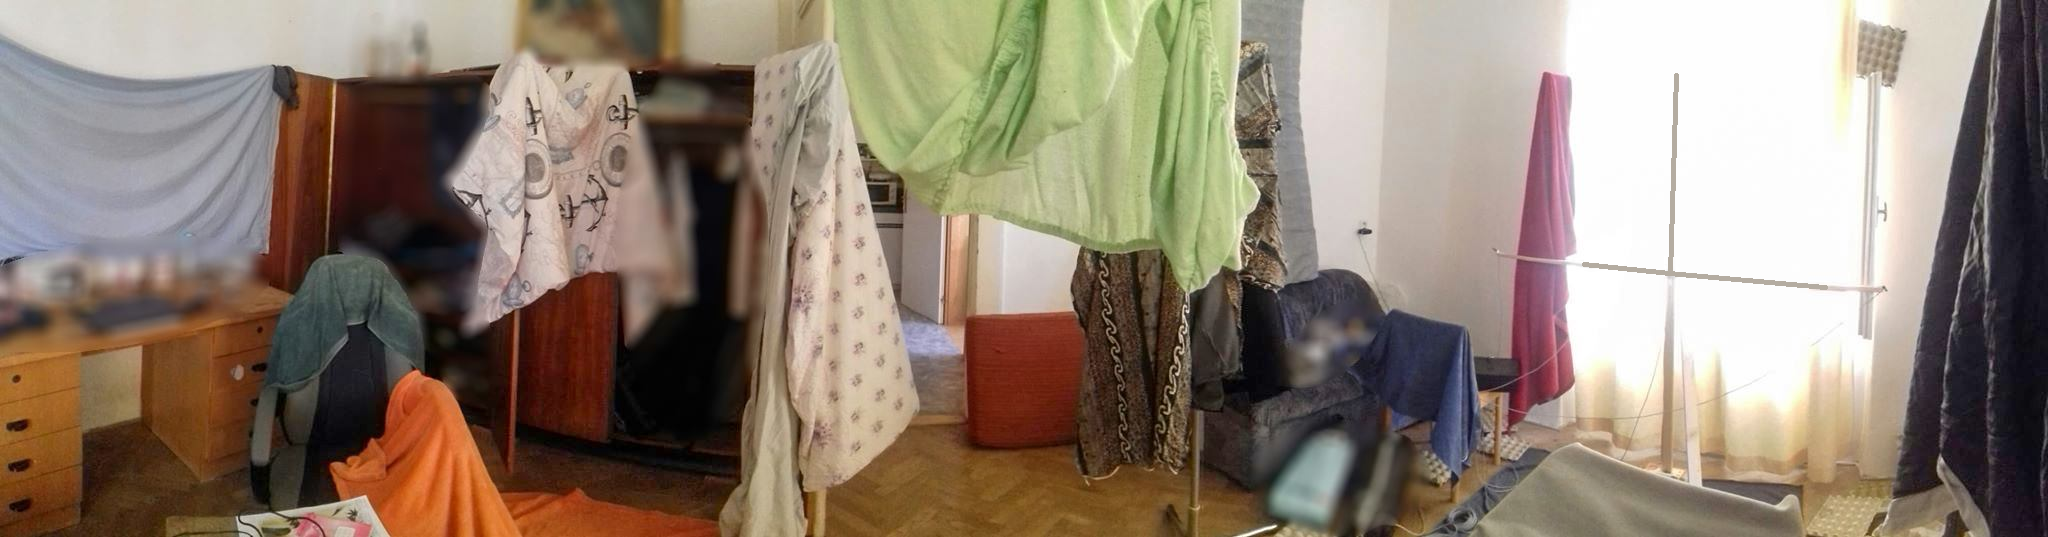
\includegraphics[width=0.9\textwidth]{obrazky-figures/neporadek.png}
	\caption{Fotografie zachycuje přibližně 180\degree \ panorama zatlumené místnosti. Na pravé straně je vidět prototyp nahrávacího kříže, který byl na tento test využit.}
	\label{pic:neporadek}
\end{figure}
\newpage
\subsection{Prostorový aliasing}
\label{aliasing}

Prostorový aliasing teoreticky znemožňuje zachycení většiny řečových frekvencí, ale nepočítá s~možností, že zpracovávané okno bude dostatečně dlouhé, aby pojalo celou délku tónu, tím se zajistilo, že správný posun signálů bude mít určitě vyšší hodnotu korelačního koeficientu než špatný posun. Takto vypočtená korelace je znázorněna na grafu \ref{pic:graf:alias}. Problém by nastal například u~hudby, kde by během nahrávaného vzorku byla tato frekvence skrz celou počítanou část. Korelace by však měla zaznamenat jakoukoli změnu, a tudíž by aliasing vadil jen v~případě naprosto harmonického signálu nebo při výpočtu s~příliš krátkými okny. V~praxi však aliasing má vliv na nepřesně určenou korelaci. Příklad, kde aliasing teoreticky nevadí, je znázorněn na obrázku \ref{pic:graf:alias}, kde generovaný harmonický signál je zachycen celý v~jednom vzorku. Délka signálu odpovídá přibližně jedné slabice ve slově.

\begin{figure}[!ht]
	\centering
	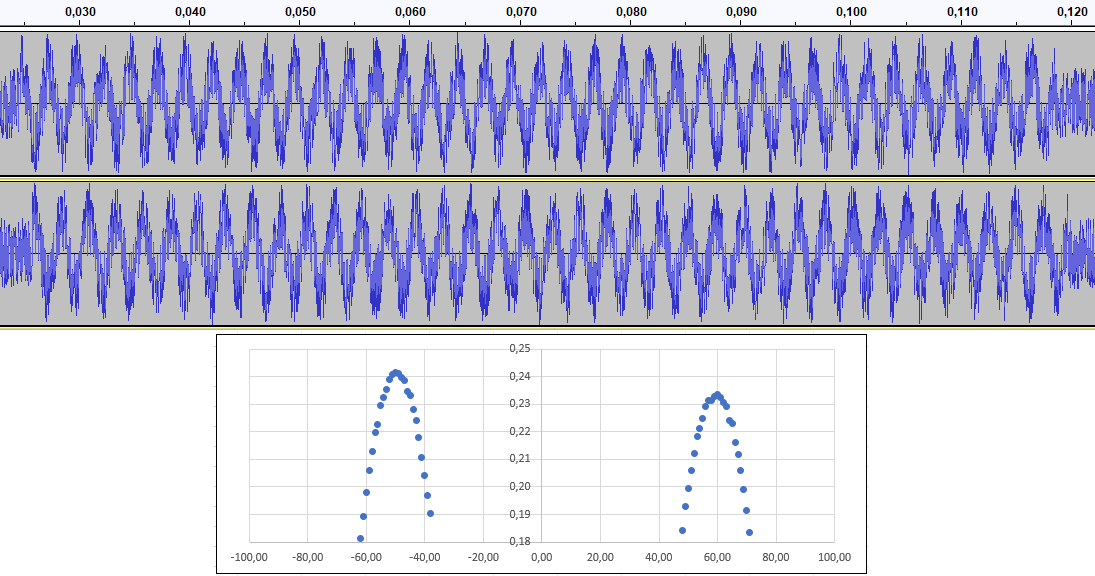
\includegraphics[width=1\textwidth]{obrazky-figures/korelAliasing.png}
	\caption{Obrázek ukazuje dva porovnávané generované signály a výpočet korelací. Správný posun je o~50 vzorků dolního signálu doleva. Graf ukazuje viditelný rozdíl i přes prostorový aliasing.}
	\label{pic:graf:alias}
\end{figure}

Prostorový aliasing lze redukovat dvěma způsoby. První možností je v~mikrofonním poli umístit mikrofony blíže k~sobě, to však má za následek menší rozptyl zpoždění signálů, a tudíž i menší přesnost určení polohy. 

Druhá možnost je počítat s~delšími okny, tím dokážeme počítat s~celým harmonickým signálem a efekt bude podobný jako na generovaném signálu, který je znázorněn na již zmiňovaném grafu \ref{pic:graf:alias}. Tato operace naopak zvyšuje výpočetní náročnost. Také je třeba počítat s~možností pohybu zdroje zvuku během nahrávky. Pohyblivý zdroj zapříčiní rozdílnou korelaci již v~jednom okně a další možnost zvětšení chyby.

Aliasing teoreticky neovlivní výpočet natolik, aby znehodnotil výpočet. Problém však nastává v~kombinaci s~ozvěnou. Odražený signál zvýší amplitudu aliasingu a tím se vyhodnotí špatný posun. Při takové chybě nevzniká chyba v~určení polohy pouze několik centimetrů, ale může se jednat i o~několik metrů. 

\subsection{Délka korelovaných signálů}

Délka okna může velmi mít neblahý dopad vlivem aliasingu na výsledek korelačních metod. Problém však může být také ve výkonu zvukové karty. Na počítači nemusíme dbát na optimalizaci a můžeme počítat bez problémů i s~vteřinovým oknem. U~zvukové karty je však problém, že DSP jádra a ALSA driver nemají možnost většího zásobníku, než je právě 6144 rámců (při použití 5 mikrofonů). Proto by byla jediná možnost uchovávat si tento zásobník v~programu ale to by zatížilo výpočetní procesor. V~ideálním případě by mělo být možné počítat s~okny o~délce 6144 rámců.

Délka okna má vliv na přesnost i kvůli přesahu signálů. Počítá se s~přesahem signálů 139 vzorků na obě strany. Předpokládejme, že první signál není vůči druhému signálu posunutý. V~případě, že se v~dalších 139 vzorcích nachází velký energetický nárůst (například začátek slova), pak se může stát, že korelace vyhodnotí posun směrem k~tomuto nárůstu oproti neposunutým signálům. Tento případ je ilustrován na obrázku \ref{pic:chybakorelace}. Řešením je dostatečně dlouhé okno, aby tento nárůst neměl větší vliv na celou nahrávku než hledaný signál.

\begin{figure}[!ht]
	\centering
	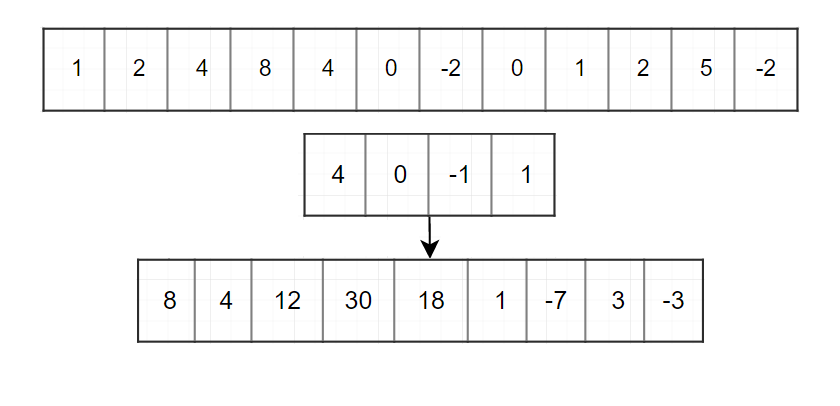
\includegraphics[width=0.8\textwidth]{obrazky-figures/5.png}
	\caption{Znázorněna správná korelace s~výskytem nárůstu v~přesahu (hodnota 8 na horním signálu), která zapříčiňuje vyšší hodnotu korelace na špatné pozici (hodnota 30 na dolních výsledcích korelace).}
	\label{pic:chybakorelace}
\end{figure}

Příklad vlivu délky rámce na výsledek, při výpočtu s~reálnými nahrávkami, je na grafech \ref{pic:delkaokna}.

\begin{figure}[!ht]
	\centering
	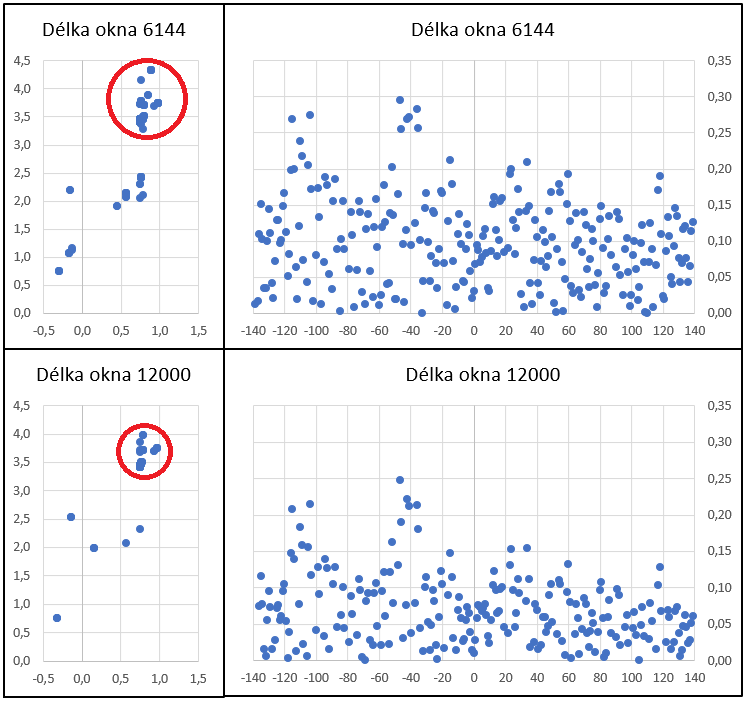
\includegraphics[width=0.8\textwidth]{obrazky-figures/vliv_delky_okna.png}
	\caption{Na grafech je znázorněn výpočet pro zdroj zvuku na souřadnicích [1,0,4]. V~horní polovině jsou grafy při výpočtu s~délkou okna 6144, v~červeném kruhu je 79,9 \% všech hodnot. V~dolní polovině jsou grafy při výpočtu s~délkou okna 12000 rámců. Zde je v~červeném kruhu 89,2 \% hodnot.}
	\label{pic:delkaokna}
\end{figure}

Tabulka \ref{tabulka2} ukazuje rozdílnou úspěsnost určení přibližné polohy při různých délkách okna. Sloupce jsou jednotlivé testy a řádky různé délky oken:

\begin{table}[!h]
    \centering
    \begin{tabular}{||c | c | c | c||} 
 \hline
 & [0,0,2] & [0,0,3] & [1,0,4] \\ [0.5ex] 
 \hline
 6144 & 83 \% & 45 \% & 17 \% \\ 
 \hline
 12000 & 87 \% & 53 \% & 33,5 \% \\
 \hline
 24000 & 80 \% & 44 \% & 35 \% \\
 \hline
 32000 &  & 33 \% & 54 \% \\
 \hline
 48000 &  & 19 \% & 22 \% \\ [1ex] 
 \hline
    \end{tabular}
    \caption{Úspěšnost určení přibližné polohy při různých délkách okna.}
    \label{tabulka2}
\end{table}
\newpage

\subsection{Nepřesná poloha zdroje zvuku vůči mikrofonnímu poli}

Poloha zdroje zvuku zapříčiněná nepřesným měřením nejspíš ovlivnila výsledek testu na obrázku \ref{pic:test2}. Shluk je vidět přibližně o~dvacet centimetrů bokem, než byl test zamýšlen.
Naštěstí tento problém není třeba řešit, protože zasahuje pouze do experimentální roviny, ale na přesnosti chodu aplikace nemá později vliv.

\subsection{Nepřesná rychlost zvuku v~aktuálních podmínkách}

Ve výpočtech je používaná rychlost zvuku při 20 \degree C 343 $ms^{-1}$. V~místnosti však stačí, aby byla teplota 19 \degree C a při této teplotě bude rychlost zvuku 342 $ms^{-1}$. Vliv na výpočet je vidět v~tabulce \ref{tabulka3}.

\begin{table}[!h]
    \centering
    \begin{tabular}{||c | c | c | c||} 
 \hline
 x (cm) & y (cm) & z~(cm) & rychlost zvuku ($ms^{-1}$) \\ [0.5ex] 
 \hline\hline
 -19.5620 & -19.8197 & 296.8366 & 350 \\ 
 \hline
 -19.5489 & -19.7964 & 303.3376 & 343 \\
 \hline
 -19.5471 & -19.7931 & 304.2872 & 342 \\
 \hline
 -19.5452 & -19.7898 & 305.2423 & 341 \\
 \hline
 -19.5434 & -19.7865 & 306.2027 & 340 \\ [1ex] 
 \hline
    \end{tabular}
    \caption{Různý výpočet polohy ze stejných dat s~rozdílně zvolenou rychlostí zvuku.}
    \label{tabulka3}
\end{table}


Rozdíly jsou v~řádech maximálně jednotek centimetrů, proto lze tento problém minimálně v~této práci zanedbat. Jako prostor pro zlepšení to však stále je a pro výpočet na větší vzdálenosti je naopak žádoucí pracovat i s~rychlostí zvuku, protože se vzdáleností se tato chyba zvyšuje.

\subsection{Slabé a nedostatečně kvalitní mikrofony}

Mikrofony jsou zásadní komponentou v~celém systému. Pokud jsou mikrofony nekvalitní, není možné vylepšit výsledky. Naštěstí mikrofony, které byly k~experimentům zapůjčeny jsou dostatečně kvalitní pro účely určení polohy zdroje zvuku v~obytné místnosti. Kvalitnějšími mikrofony a mikrofony s~jinou směrovou charakteristikou a citlivostí by přineslo zpřesnění výpočtu a vylepšení celkového výsledku práce.

\subsection{Nepřesné umístění mikrofonů v~mikrofonním poli}

Jako poslední příčina možné chyby ve výpočtu je nepřesně sestavené mikrofonní pole. Jako příklad je uveden obrázek \ref{pic:mikrofon_posun}, kde byl na jedné ose posunut mikrofon o~1 cm dál od středového. Jedna správná hyperbola mezi mikrofony 1 metr vzdálenými a jedna posunutá hyperbola mezi mikrofony vzdálenými 1,01 metru se následně střetly v~bodě [-0,0025,2,9847]. Správný bod střetnutí je [0,3]. Rozdíl mezi těmito body je 1,55 cm. Tato chyba se dá považovat za dostatečně malou, abychom ji mohli zanedbat.

\begin{figure}[hbt]
	\centering
	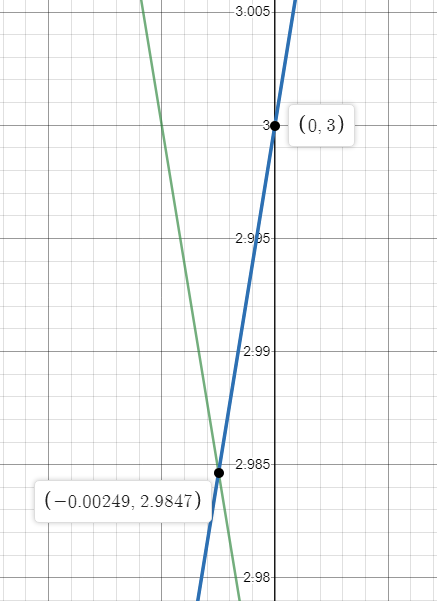
\includegraphics[width=0.4\textwidth]{obrazky-figures/nepresne_mik_pole.png}
	\caption{Na grafu je průsečík modré hyperboly, která má mikrofony přesně 1 metr vzdálený a zpoždění signálů odpovídá zdroji na pozici [0,3], a zelené hyperboly, která má mikrofony vzdálené 1,01 metru a počítá se se vzdáleností 1 metr (chyba 1 cm).}
	\label{pic:mikrofon_posun}
\end{figure}
%\footnote{Graf vytvořen v nástroji \href{https://www.desmos.com/calculator/8ngxlbqf0r}{www.desmos.com}}

\section{Porovnání výsledků simultánního vyhodnocování polohy}

Pro běh programu na zvukové kartě v~reálném čase bylo nutné ve výpočtu přeskakovat data tak, aby nedocházelo k~nutnosti zotavení zvukové karty. Vynechávání dat při výpočtu může vést k~horším výsledkům. Proto je vhodné porovnat výsledky dosažené s~optimalizovaným systémem s~plným výpočtem na laptopu.

Testy proběhly za stejných vnějších podmínek. Zdroj byl usazen na totožném místě a hlasitost reproduktoru byla na stejné úrovni. Výjimkou byl test na reálné řeči, kdy nebylo možné dokonale zreplikovat stejný test. Test bez použití reproduktorů v~první části nahrávky obsahuje mužský hlas na souřadnicích [1,0,3] blízko zdi a posléze mužský hlas na souřadnicích [-1,0,2] uprostřed pokoje. Tento test také ukazuje, že záleží na pozici zdroje vůči zdem, od kterých se může odrážet zvuk. V~tabulce \ref{tabulka4} je uvedena procentuální úspěšnost určení správného okolí polohy. Řádky znázorňují délku okna a platformu a sloupce souřadnice pozice zdroje zvuku v~testu.

\begin{table}[!h]
    \centering
    \begin{tabular}{|| c |c | c | c | c||} 
 \hline
 & [0,0,2] & [0,0,3] & [1,0,4] & řeč \\ [0.5ex] 
 \hline
 RT 6144 & 82 \% & 42,5 \% & 29 \% & 74 \% \\ 
 \hline
 PC 6144 & 83 \% & 45 \% & 17 \% & 61 \% \\
 \hline
 PC 12000 & 87 \% & 53 \% & 33,5 \% & 63 \% \\
 \hline
 PC 24000 & 80 \% & 44 \% & 35 \% & 72,5 \% \\ [1ex] 
 \hline
    \end{tabular}
    \caption{Správné určení přibližné polohy zdroje zvuku při různé délce okna a při různých testech. RT (real-time) - běh v~čase na zvukové kartě. PC – běh bez optimalizace na laptopu.}
    \label{tabulka4}
\end{table}

Na grafu výsledků \ref{pic:rec_chyba} při testování, je dobře poznat vliv odrazu od zdi v~kombinaci s~aliasingem. V~tomto testu na pozici 1 a 2 jsou správně vypočtené polohy dvou různých řečníku a na pozici 3 je shluk vypočtených souřadnic pravděpodobně ovlivněných aliasingem a odrazem od zdi.

\begin{figure}[hbt]
	\centering
	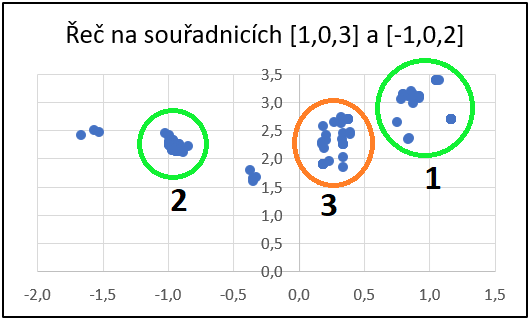
\includegraphics[width=0.6\textwidth]{obrazky-figures/rec_chyba.png}
	\caption{Výsledky vypočtené polohy dvou řečníků na souřadnicích [1.0,3] a [-1,0,2]. Příklad vlivu odrazu zvuku a aliasingu.}
	\label{pic:rec_chyba}
\end{figure}

\chapter{Závěr}

V~první polovině roku jsem studoval vlastnosti zvuku a způsoby zaznamenávání audio signálů. Seznámil jsem se s~mikrofonním polem a sestrojil jsem prototyp mikrofonního pole. Vymyslel jsem algoritmus výpočtu pomocí hyperbol a implementoval jsem ho. Signály jsem koreloval běžnou metodou kartézského součinu dvou signálů. V~polovině zimního semestru mi byla zapůjčena školou sestava systému ARM/SHARC, pomocí které jsem nahrál testovací nahrávky pro prvotní testování svých algoritmů.

V~druhé polovině roku jsem zjistil nepřesnosti ve výpočtech a vlivy na výsledek. Pořídil jsem nové nahrávky v~zatlumené místnosti, neboť ozvěna měla zásadní vliv na určení polohy. Upravil jsem korelační metodu na normalizovanou křížovou korelaci a pro srovnání naprogramoval také korelace odečítáním signálů. Prováděl jsem testování jednotlivých částí programu, aby byla odhalena jeho nejslabší část. Zjistil jsem, že výpočet energie je spolehlivý, ale je nutné zvyšovat koeficient podle požadované maximální vzdálenosti od mikrofonů a také podle kvality mikrofonů. Frekvenční filtrace signálů není třeba, neboť nebyl prokázán pozitivní vliv na výsledky výpočtů. Jako kámen úrazu se ukázal výpočet korelace, který byl závislý převážně na vnějších vlivech. Po experimentech s~parametry spouštěného programu a výpočtech na různých nahrávkách jsem si dovolil definovat zásady pro spolehlivější chod programu:

\begin{itemize}
  \item Zamezení vzniku ozvěny v~místnosti.
  \item Čím delší výpočetní okno, tím lepší korelace. Oproti tomu čím kratší výpočetní okno, tím přesnější a rychlejší určení pohybujícího se zdroje.
  \item Energetický práh je na velmi krátkou vzdálenost ideální přibližně 4. Naopak pro větší vzdálenosti zdroje zvuku více jak dva metry a při tiché řeči je dobré počítat s~prahem 2,5, případně nižší.
  \item Řečník by měl mluvit směrem k~mikrofonnímu poli a dostatečně nahlas.
  \item Použití přesného mikrofonního pole s~dostatečným odstupem od bočních zdí, ideálně připevněné na tlumícím materiálu.
  \item Možný prostor pohybu zdroje zvuku je znám před spuštěním programu.
  \item Zdroj zvuku se nevyskytuje blízko zdí.
  \item Pokud možno v~zaznamenávaném prostoru nevzniká šum a zdroj zvuku je v~jednu chvíli pouze jeden.
  \item Rychlost zvuku v~místnosti je 343 $ms^{-1}$.
\end{itemize}

Při zajištění všech těchto podmínek by bylo možné s~jistotou určit zdroj zvuku i na větší vzdálenost než 3 metry. Mé možnosti však byly omezené, a proto testování nebylo možné na větší vzdálenost než 4 metry.

Přínos mé práce je ve zjištění, které vlivy na určení polohy mají vliv a jaký. Zjistil jsem jaký vliv má rozdílná rychlost zvuku ve vzduchu a že může ovlivnit výpočet polohy již 3 metry vzdáleného zdroje od mikrofonního pole o~téměř 10 centimetrů. Chybně sestavené mikrofonní pole ovlivní výpočet jen o~jednotky centimetrů. Prostorový aliasing nemusí nutně znamenat chybný výpočet korelace, a naopak v~kombinaci s~ozvěnou dokáže dokonale znehodnotit výsledky. Znázornil jsem rozdíl mezi výpočtem s~vzorkovací frekvencí 8 kHz a 48 kHz a tím i ukázal, že vypočítat vzdálenější polohu menší vzorkovací frekvencí je téměř nemožné.

Aplikace dokáže správně určit pozici řečníka na vzdálenost tří metrů s~chybovostí přibližně 20 \%.

\section{Možnosti budoucí práce a vylepšení}

Jak už několikrát bylo zmíněno, největší vliv na správné určení polohy měla ozvěna vznikající v~místnosti. Pokud by se podařilo tuto ozvěnu odfiltrovat v~programu, mohl by se systém aplikovat do jakékoli i nezatlumené místnosti.

Další možnost vylepšení je lepší hardware. Výpočetní výkon ARM jádra na zvukové kartě není dostatečný pro výpočet korelace s~vzorkovací frekvencí 48 kHz. Zlepšení výkonu lze dosáhnout buď využitím DSP jádra nebo jiného hardwaru nebo další optimalizace algoritmů. Při vylepšení hardwaru je vhodné pořídit i kvalitnější mikrofony s~kardioidní směrovou charakteristikou. Optimalizovat program by bylo možné například paralelismem. Výpočet by pak mohl probíhat v~době, kdy systém neregistruje řeč.

Pokud by byla možnost lepšího výpočetního výkonu, šlo by také využít dalších mikrofonních polí. Ve větších místnostech přidat mikrofonní pole na zdi na opačných stranách nebo případně pro odhadnutí přibližné polohy použít menší mikrofonní pole a násladně větším mikrofonním polem toto místo určit přesněji.

Korelační metoda, kterou jsem využil nepracuje ve frekvenčním spektru a není otestováno, zda korelační metody využívající Fourierovu transformaci by nemohly být lepší. Bylo by vhodné tyto metody v~budoucnu otestovat.

Má práce pracuje se statickým výpočtem korelace z~mikrofonního pole 2x2 metry. Tento algoritmus by mohl být přepracován a zobecněn pro výpočet v~různě velkých mikrofonních polí. Po zmenšení mikrofonního pole se zmenší přesnost určení polohy, ale zároveň se redukuje účinek prostorového aliasingu na korelační metody.

Je použito zjednodušení vlivu rychlosti zvuku ve vzduchu na statických 343 $ms^{-1}$. V~práci je popsáno, jak se tato rychlost vypočítá a při předpokladu běžného tlaku lze počítat tuto rychlost pouze v~závislosti na teplotě vzduchu. Přidáním elektronického teploměru do tohoto systému by se zajistila další přesnost. Tato úprava by měla vliv hlavně pro výpočet vzdálenější polohy zdroje zvuku.

Výsledku této práce by se dalo využít například, jak bylo uvedeno již v~úvodu, k~zaměřování osvětlovacího systému, případně kamer na zdroj zvuku – řečníka.
